%%%%%%%%%%%%%%%%%%%%%%%%%%%%%%%%%%%%%%%%%%%%%%%%%%%%%%%%%%%%%%%%%%%%%%%%
% Plantilla TFG/TFM
% Escuela Politécnica Superior de la Universidad de Alicante
% Realizado por: Jose Manuel Requena Plens
% Contacto: info@jmrplens.com / Telegram:@jmrplens
%%%%%%%%%%%%%%%%%%%%%%%%%%%%%%%%%%%%%%%%%%%%%%%%%%%%%%%%%%%%%%%%%%%%%%%%

\chapter{Antenas Microstrip}
\label{antenasmicrostrip}

\section{Introducción}
\par Las antenas de parche o antenas microstrip son un tipo de antenas de tipo planar que utilizan la tecnología microstrip para su funcionamiento. En el año 1953 \textit{G. A. Deschamps} y \textit{W. Sichak} presentaron ante el Tercer Simposio sobre Investigación y Desarrollo de Antenas organizado por las Fuerzas Aéreas de los Estados Unidos su trabajo "Microstrip Microwave Antennas" (Antenas de Microondas Microstrips), lo que se considera como el primer \textit{paper} sobre este tipo de antenas, pero no fue hasta dos décadas más tarde, en 1970 cuando, gracias al desarrollo de los \gls{pcb}, se pudieron empezar a realizar los primeros desarrollos de líneas de transmisión y antenas con tecnología microstrip. Desde entonces, las antenas microstrip se han convertido en uno de los tipos de antena más usado para un alto abanico de aplicaciones. \cite{Bernhard2003, Balanis2015} 
\\
\par Entre sus principales ventajas se encuentra su delgadez y capacidad de adaptación a distintos tipos de superficies, incluso pudiendo ser conformadas en superficies curvas y no planares. Además son antenas simples, muy ligeras, fáciles de diseñar, con un coste de producción bajo, fáciles de transportar, y preparadas para ser integradas en arrays. Por estas razones, los circuitos y antenas microstrip son comúnmente usados para la fabricación de circuitos monolíticos integrados para microondas (MMICs) en aplicaciones civiles, militares, gubernamentales y comerciales como identificación por radio frecuencia (RFID), retransmisión de radio, sistemas de comunicaciones móviles, \gls{gps}, televisión, comunicaciones satelitales (fig. \ref{fig:satgalileo}), sistemas de vigilancia, radar, y guiado de misiles entre otros. \cite{Aquino2008} 
\\
\par Por otra parte, las antenas microstrip son muy versátiles en términos de resonancia y polarización, con obtención de buenos patrones de radiación y fácil adaptación de impedancias. Si además sumamos al circuito elementos adaptativos como diodos varicap, se pueden llegar a diseñar antenas microstrip con frecuencias, impedancias, y patrones de radiación variables. En contra, el uso de antenas microstrip conlleva ciertas limitaciones como su alto factor de calidad (Q), necesidad de limitar la potencia que atraviesa el circuito, baja eficiencia, baja pureza de polarización y ancho de banda limitado. En ciertas aplicaciones, estas limitaciones pueden ser usadas a favor, como el hecho de tener bajos anchos de banda puede ser deseado a la hora de usar las antenas microstrip en aplicaciones de seguridad gubernamental puesto que se limita el rango de penetración externa por parte de posibles atacantes.

\begin{figure}[h]
    \centering
        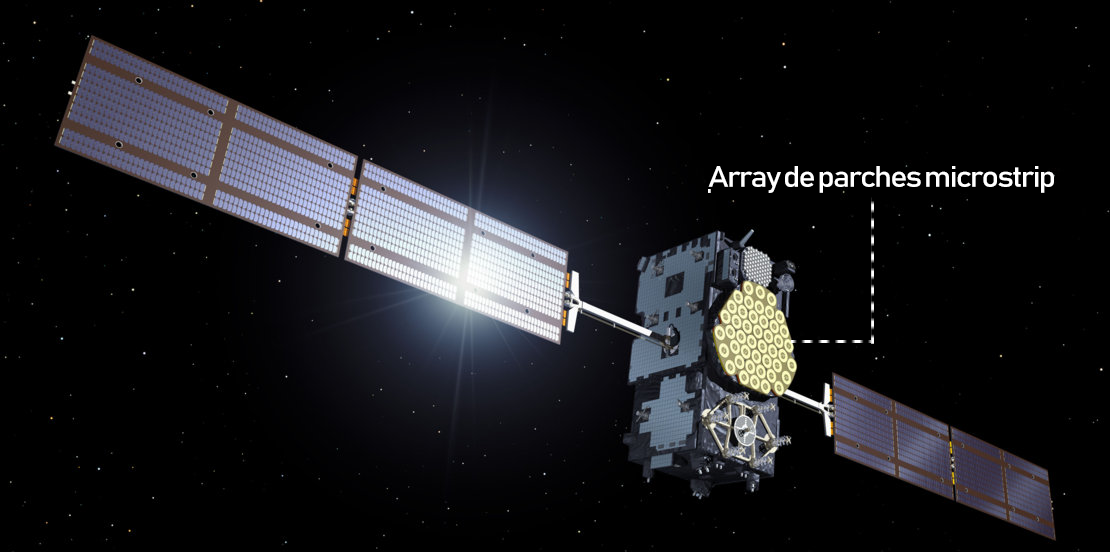
\includegraphics[width=15cm]{archivos/sate}
        \caption{Satélite IOV Galileo. \citep{Pippes2011}}
        \label{fig:satgalileo}
\end{figure}

\section{Características básicas}

\par Las antenas microstrip están formadas por tres elementos básicos: Una capa conductora muy fina, hasta tres órdenes de magnitud menor a la longitud de onda en el espacio de la señal que se desea transmitir por ella, a la que denominaremos como parche. Este arreglo metálico está situado a, aproximadamente, la centésima parte de la longitud de onda en el espacio, del plano de tierra o masa de la antena, que consistirá en una superficie metálica normalmente, del mismo grosor que el parche. Para que un parche rectangular resuene a una frecuencia concreta, la longitud de este debe ser de entre la mitad y un tercio de la longitud de onda de la señal deseada.
\\
\par Entre el parche y el plano de masa se sitúa el dieléctrico o substrato, encargado de aislar ambos materiales previamente mencionados. El substrato se caracteriza por su permitividad relativa o constante dieléctrica ($\epsilon_{r}$), y para la construcción de antenas microstrip, esta suele oscilar entre valores de 2.2 y 12. Cuanto más grueso sea el substrato, mejores resultados respecto a ancho de banda y eficiencia obtendremos en el diseño, sacrificando la pérdida de espacio ocupado por el substrato correspondiente, la cual puede ser muy limitada en ciertas aplicaciones. Por otro lado, substratos finos con valores de permitividad relativa alta son usados para aplicaciones de microondas ya que estas requieren contornos muy finos para evitar radiaciones indeseadas y acoplamientos.
\\
\par Normalmente, las antenas microstrip están integradas en otros circuitos de microondas, con lo que es necesario llegar a un compromiso entre las características de diseño requeridas por la aplicación y el buen rendimiento de la antena. Además de parches rectangulares, las antenas microstrip pueden tomar diversidad de formas para adaptarse a las limitaciones de diseño especificadas por la aplicación. Entre las formas más comunes que toman las antenas microstrip se encuentran cuadrados, círculos, elipses, sectores circulares, triángulos, o dipolos. Este tipo de diseños pueden ayudarnos a mejorar ciertas características relacionadas con la radiación de la antena o la adaptación de ésta dentro de sistemas más complejas. Otro método para conseguir este tipo de mejoras, así como para poder aumentar el ancho de banda o la directividad es el uso de arrays de antenas microstrip. 
\\
\par Las características de sintonización y adaptación de las antenas de parche microstrip residen principalmente en las dimensiones de los elementos que la componen. En la figura \ref{fig:elementos} se puede observar cómo se organiza una antena microstrip de un solo elemento y las denominación común que se le dan a las variables que definen la dimension de estos elementos. Las variables más importantes a la hora de diseñar una antena microstrip rectangular son los siguientes:

\begin{itemize}
\item \textbf{L: }Longitud del parche
\item \textbf{W: }Anchura del parche
\item \textbf{h: }Altura o espesor del dieléctrico
\item \textbf{t: }Altura o espesor del parche y de la tierra
\item \textbf{$\epsilon_{r}$: }Constante dieléctrica
\end{itemize}
 
\begin{figure}[h]
    \centering
        \includegraphics[width=15cm]{archivos/parche/elemento}
        \caption{Partes de una antena microstrip.}
        \label{fig:elementos}
\end{figure}

\section{Ondas en antenas microstrip}

\par Durante el proceso de normal funcionamiento de las antenas microstrip, diferentes tipos de ondas pueden aparecer en sus líneas y superficies. Algunas de estas ondas son indeseadas puesto que pueden causar interferencias sobre los campos eléctricos que proceden del generador que se haya instalado, y es de vital importancia diseñar la la antena de forma que su aparición sea mínima. Existen cuatro tipos de ondas principales: \cite{Aquino2008}

\begin{itemize}
\item \textbf{Ondas espaciales: }Estas tipo de \gls{oem} son las que serán radiadas al final del proceso de funcionamiento de la antena. Estas ondas abandonarán la estructura de la antena y se propagarán en el espacio libre y se irán atenuando conforme se alejen de la antena. La propagación de estas ondas es normal y completamente deseada cuando la estructura microstrip es una antena, sin embargo, si las ondas comienzan a propagarse en la línea de alimentación de la antena, también en tecnología microstrip, significará que nuestro diseño tiene pérdidas y se deberá encontrar una solución a este problema de fugas.

\item \textbf{Ondas superficiales: }Las ondas superficiales producen pérdidas que limitan el rendimiento de la línea de transmisión o de la antena. Suelen aparecer en substratos gruesos y normalmente debido a la diferencia de densidades entre dos medios que se intentan conectar. Estas ondas se quedan atrapadas entre los dos medios debido a efecto reflexivos sin llegar a ser radiadas, lo que se conoce como "reflexión interna total". Estas ondas suelen quedar atrapadas en los substratos de las antenas microstrip y producen acoplamientos que disminuyen su rendimiento. En el caso de que estas ondas llegaran a los límites de la estructura de la antena, estas podrían llegar a ser radiadas por efectos difractivos en los ejes, lo que supondría una posible interferencia con las ondas radiadas por la antena, y la consecuente degradación del rendimiento y patrón de radiación de la antena.

\item \textbf{Ondas guiadas: }Este tipo de ondas aparecen cuando la tira microstrip está siendo usada como línea de transmisión o guía de onda. Estas ondas comienzan a viajar dentro del substrato cuando este está rellenado casi en la totalidad de su superficie por tiras microstrip eléctricas, lo que provoca que se queden rebotando entre las tiras superiores y el plano de masa.
\end{itemize}

\section{Métodos de alimentación}

\par Existen diversas maneras de alimentar una antena en tecnología microstrip. Denominamos alimentación a proceso de interconexión entre el parche y el resto del circuito integrado, incluyendo en el cualquier otro elemento pasivo, generadores, etc. Los métodos de alimentación para antenas microstrip se pueden agrupar por categorías como: Métodos de alimentación directo, alimentación por proximidad y alimentación por apertura. \cite{Aquino2008}

\subsection{Métodos de alimentación directa}
\par Los métodos de alimentación directa son aquellos en los que se interconectan físicamente las dos estructuras que componen el sistema de comunicaciones: la estructura dedicada a la alimentación, procesado y/o filtrado de la señal, y el elemento radiante. Dentro de este método de alimentación, existen dos técnicas principales: la alimentación por línea de transmisión microstrip y la alimentación por sonda coaxial.

\subsubsection{Alimentación por línea microstrip}
\par La línea de alimentación microstrip se basa en una tira de tecnología microstrip que se conecta directamente a la antena. Esta tira se caracteriza por su anchura, cuya variación definirá la impedancia que al final de la línea, verá la antena. Su espesor es igual al del parche microstrip y se sitúa, de igual manera sobre el substrato. En esta técnica de alimentación se ha de tener especial cuidado a la hora de diseñar el alimentador, puesto que ciertas configuraciones de las dimensiones de la tira pueden llevar a resonancias que propaguen la señal que se está intentando llevar a la antena. 
\\
\par Este tipo de línea es el más facil de fabricar e integrar en el circuito, además de su facilidad de adaptación de impedancias mediante el diseño del \textit{inset} o inserciones que se realizan dentro del parche para encontrar el punto donde las impedancias de la línea y la antena son idénticas y así conseguir la máxima transferencia de potencia. Entre sus limitaciones principales esta el hecho de que al aumentar el grosor del substrato aparezcan ondas superficiales y ondas espaciales, lo que en términos prácticos significa una limitación del ancho de banda del 2\% al 5\% de la frecuencia de la onda que se desea emitir.

\subsubsection{Alimentación por sonda coaxial}
\par La alimentación por línea coaxial consiste en conectar el vivo de un cable coaxial directamente al parche microstrip y su malla de tierra al plano de tierra de la antena. Este método también es sencillo de construir e implica una baja radiación espuria. También es un método que permite una fácil adaptación entre la línea y la antena, para ello se irá variando la posición de instalación de la sonda respecto al radiador de la misma forma en la que actuaban los inset en la alimentación por línea microstrip. Su principal dificultad de implementación reside en el hecho de tener que perforar el radiador para colocar y soldar el vivo del coaxial a este.

\subsection{Métodos de alimentación indirecta}
\par En estos métodos de alimentación, no existe un material conductor que toque físicamente el parche sino que este se alimentará por acoplamiento electromagnético entre un material conductor instalado cerca de él. Estos métodos de alimentación solucionan ciertas limitaciones que producen las alimentaciones directas, como el hecho de producir radiaciones con polarizaciones cruzadas.

\subsubsection{Alimentación por proximidad}
\par Para este método se hará uso de dos substratos, un substrato entre el plano superior donde se instalará el parche microstrip y un plano central donde se encontrará la línea de alimentación también en tecnología microstrip. El segundo substrato separará el plano central de alimentación con un plano de tierra situado en la parte inferior de toda la infraestructura. 
\\
\par El principio de funcionamiento se basa en el acoplamiento electromagnético entre la línea de transmisión situado como un sándwich entre los dos substratos, y el parche en la capa superior.  Las constantes dieléctricas de los distintos substratos son distintas y esto será de ayuda a la hora optimizar la penetración entre capas.
\\
\par Además, este método de alimentación permite la obtención de mejores anchos de banda, menor radiación espuria, mejor supresión del paso de modos de orden superior, y facilidad para adaptar la línea microstrip al parche. La principal desventaja de este método reside en la utilización de dos substratos, lo que incrementa notablemente el grosor del sistema de antena, lo que en ciertas aplicaciones puede no ser viable.

\subsubsection{Alimentación por ranura}
\par El método de alumentación indirecta por ranura o alimentación por apertura se basa en el principio de funcionamiento del método de alimentación por proximidad. En este método también se utilizan dos substratos, pero en una configuración distinta, en la que los planos de tierra y de alimentación, se intercambian las posiciones. Ahora en el plano inferior se encontrará la línea de alimentación microstrip mientras que en el plano central encontraremos el plano de tierra. Lo que caracteriza a este método de alimentación es que el plano de tierra central, tendrá una pequeña ranura o apertura cuyas dimensiones y posición serán claves para la adaptación de impedancias entre la línea y el parche, que seguirá instalado en el plano superior.
\\
\par Con el mismo principio de funcionamiento que la alimentación por proximidad, el parche será alimentado electromagnéticamente por la línea a través de la ranura del plano central. Este tipo de alimentación por apertura se aventaja con respecto a la alimentación por proximidad en que, al estar la línea de alimentación en el plano inferior y separada por el plano central de masa, se evitan interferencias electromagnéticas entre las radiaciones de cada plano.
\\
\par Al igual que en la alimentación por proximidad, este método de alimentación ayuda a obtener una mejor pureza de polarización, un mayor ancho de banda, y una mayor facilidad de adaptación a costa de un mayor grosor del sistema de comunicación.
\\


\begin{figure}[h]
     \centering
     \begin{subfigure}[b]{0.45\textwidth}
         \centering
         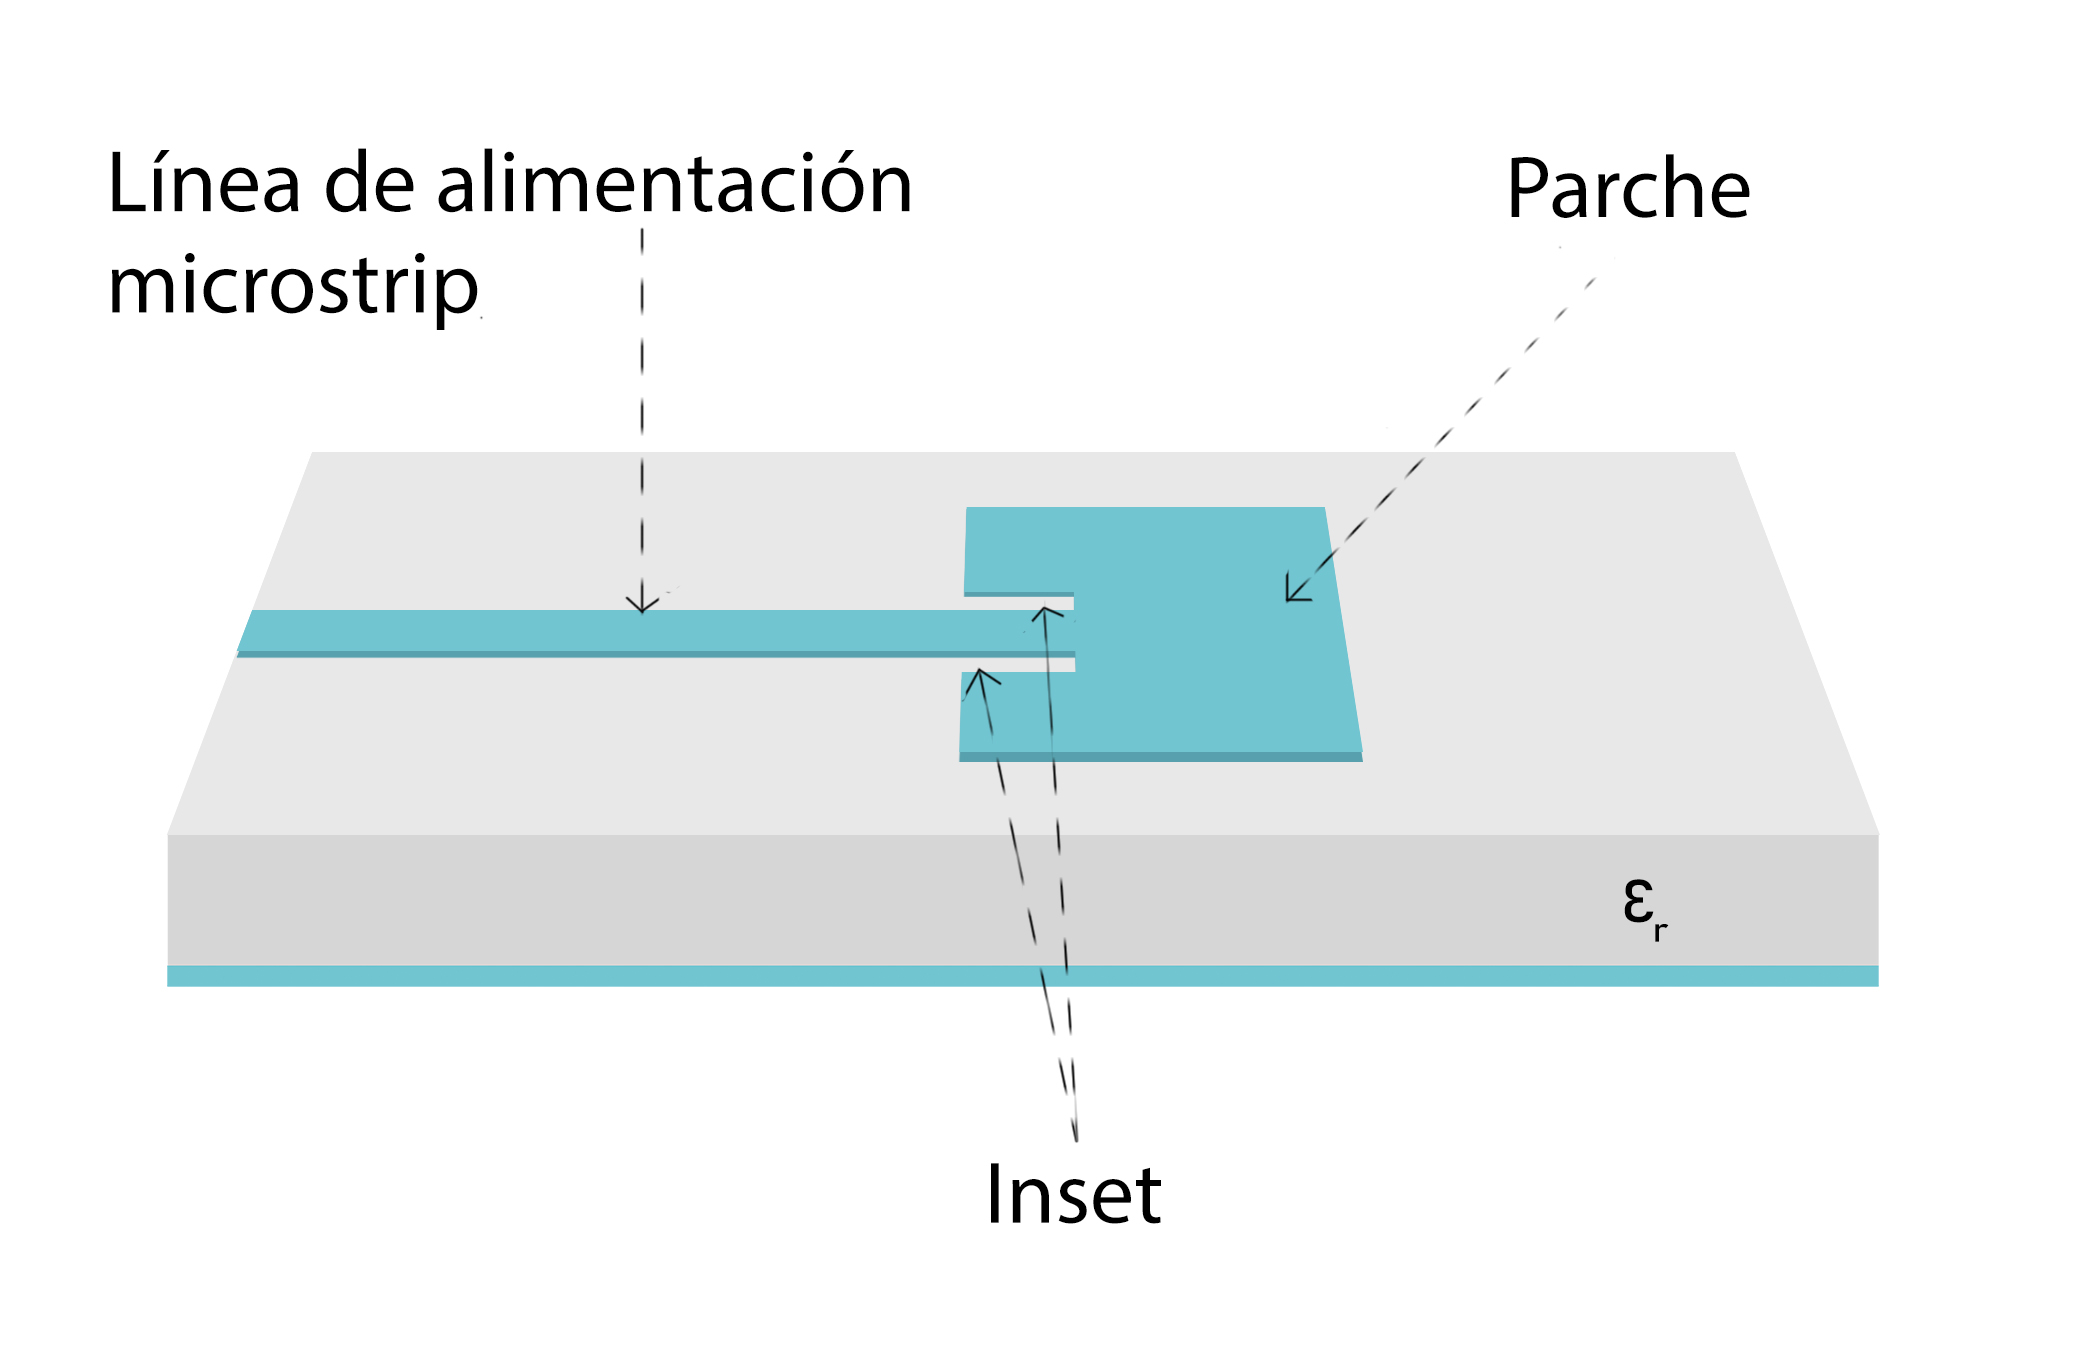
\includegraphics[width=\textwidth]{archivos/parche/directa}
         \caption{Alimentación directa}
         \label{fig:directa}
     \end{subfigure}
     \hfill
     \begin{subfigure}[b]{0.45\textwidth}
         \centering
         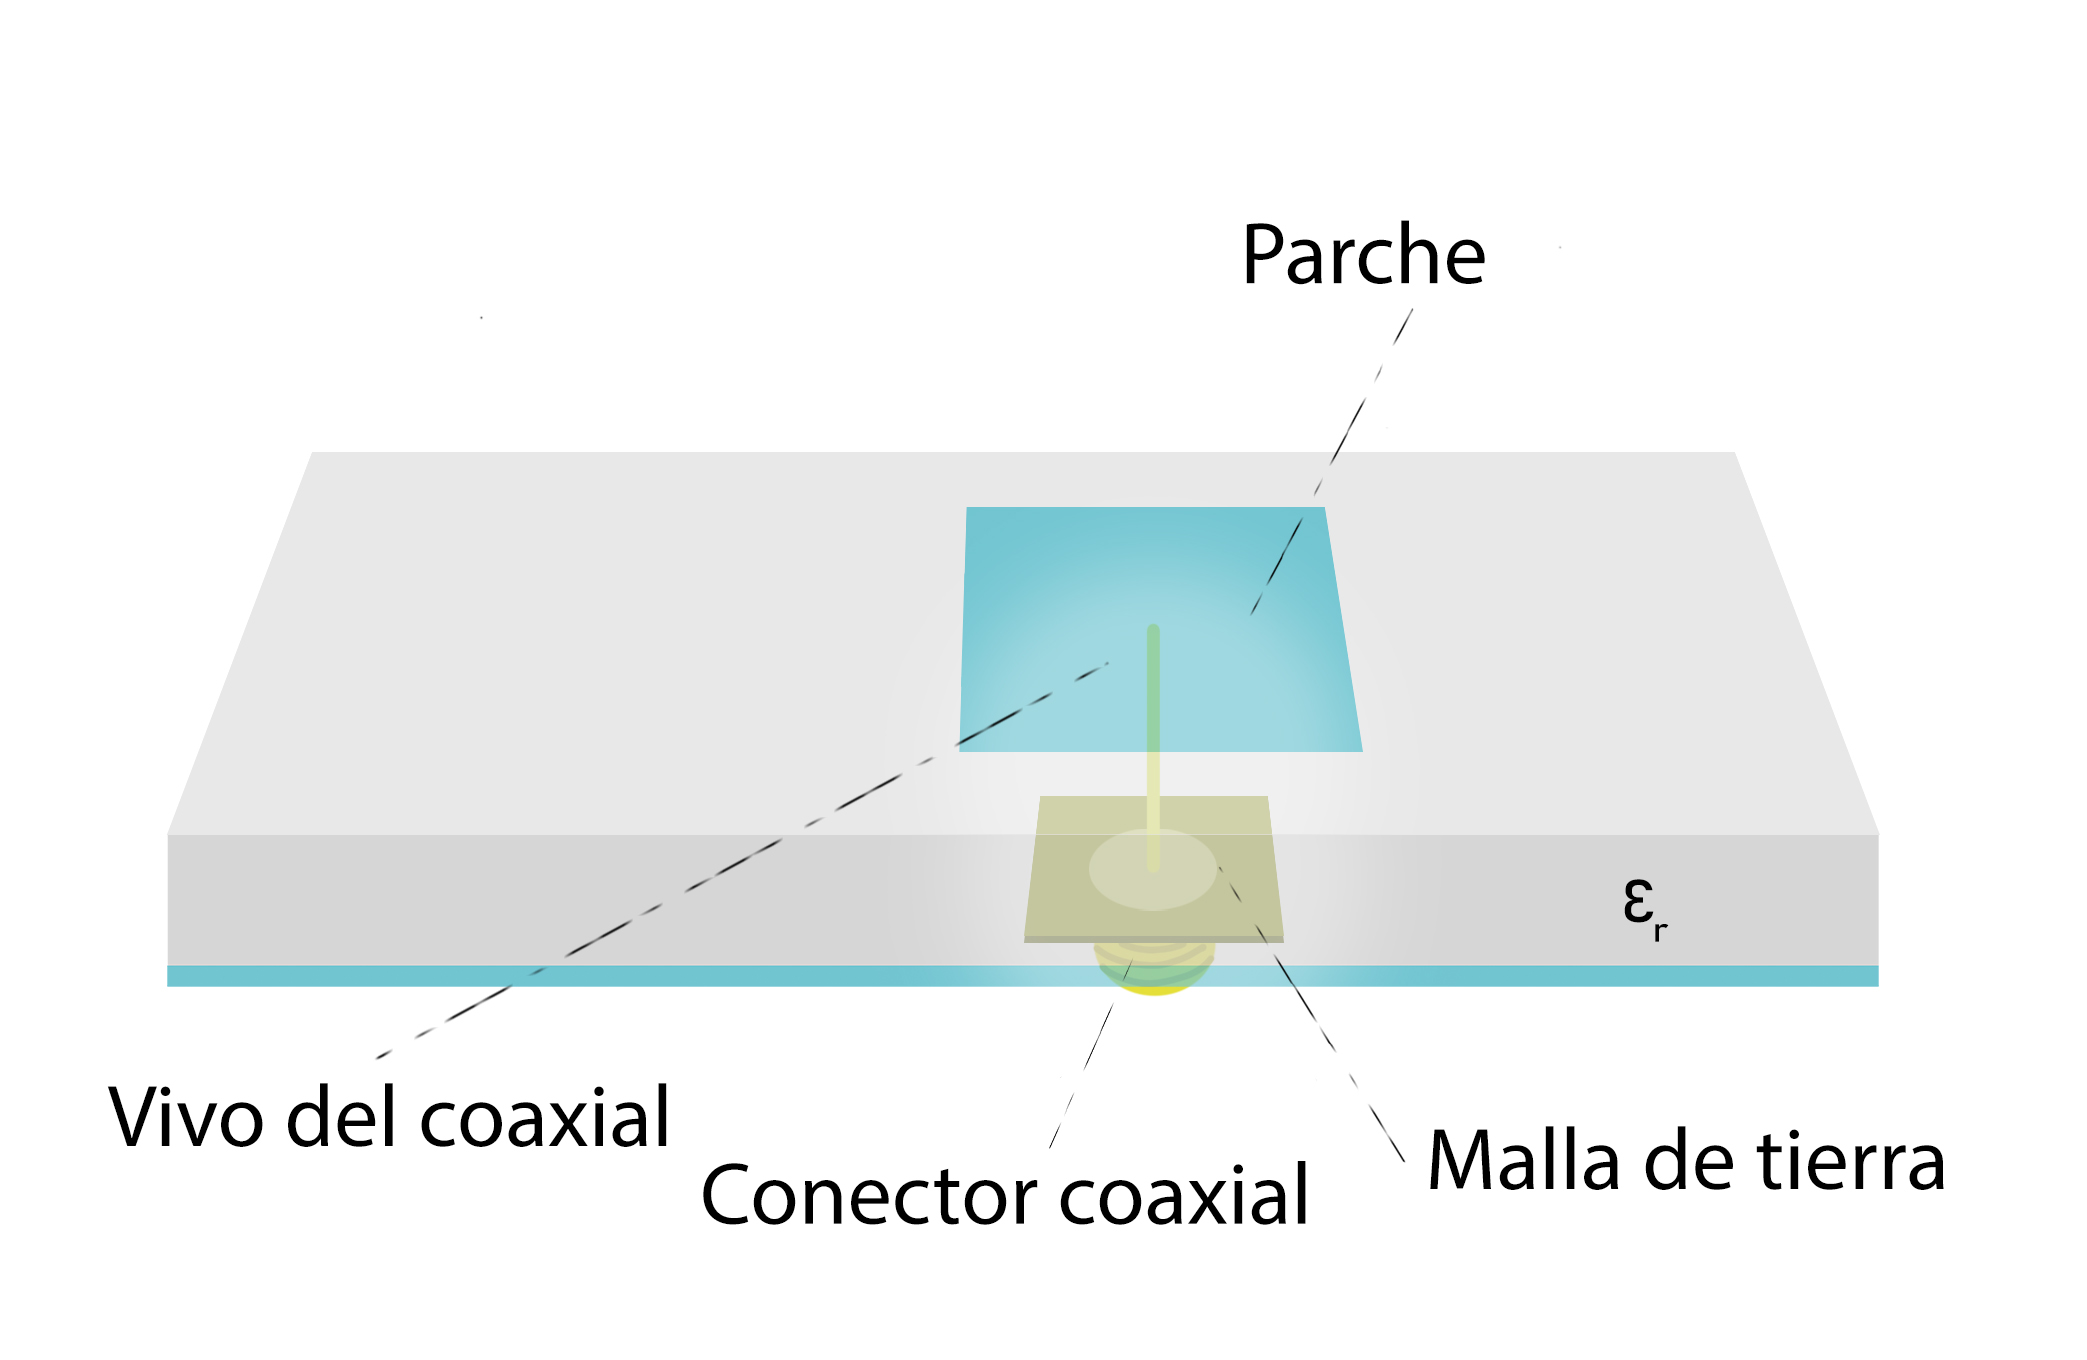
\includegraphics[width=\textwidth]{archivos/parche/coax}
         \caption{Alimentación por sonda coaxial}
         \label{fig:coax}
     \end{subfigure}
     \hfill
     \begin{subfigure}[b]{0.45\textwidth}
         \centering
         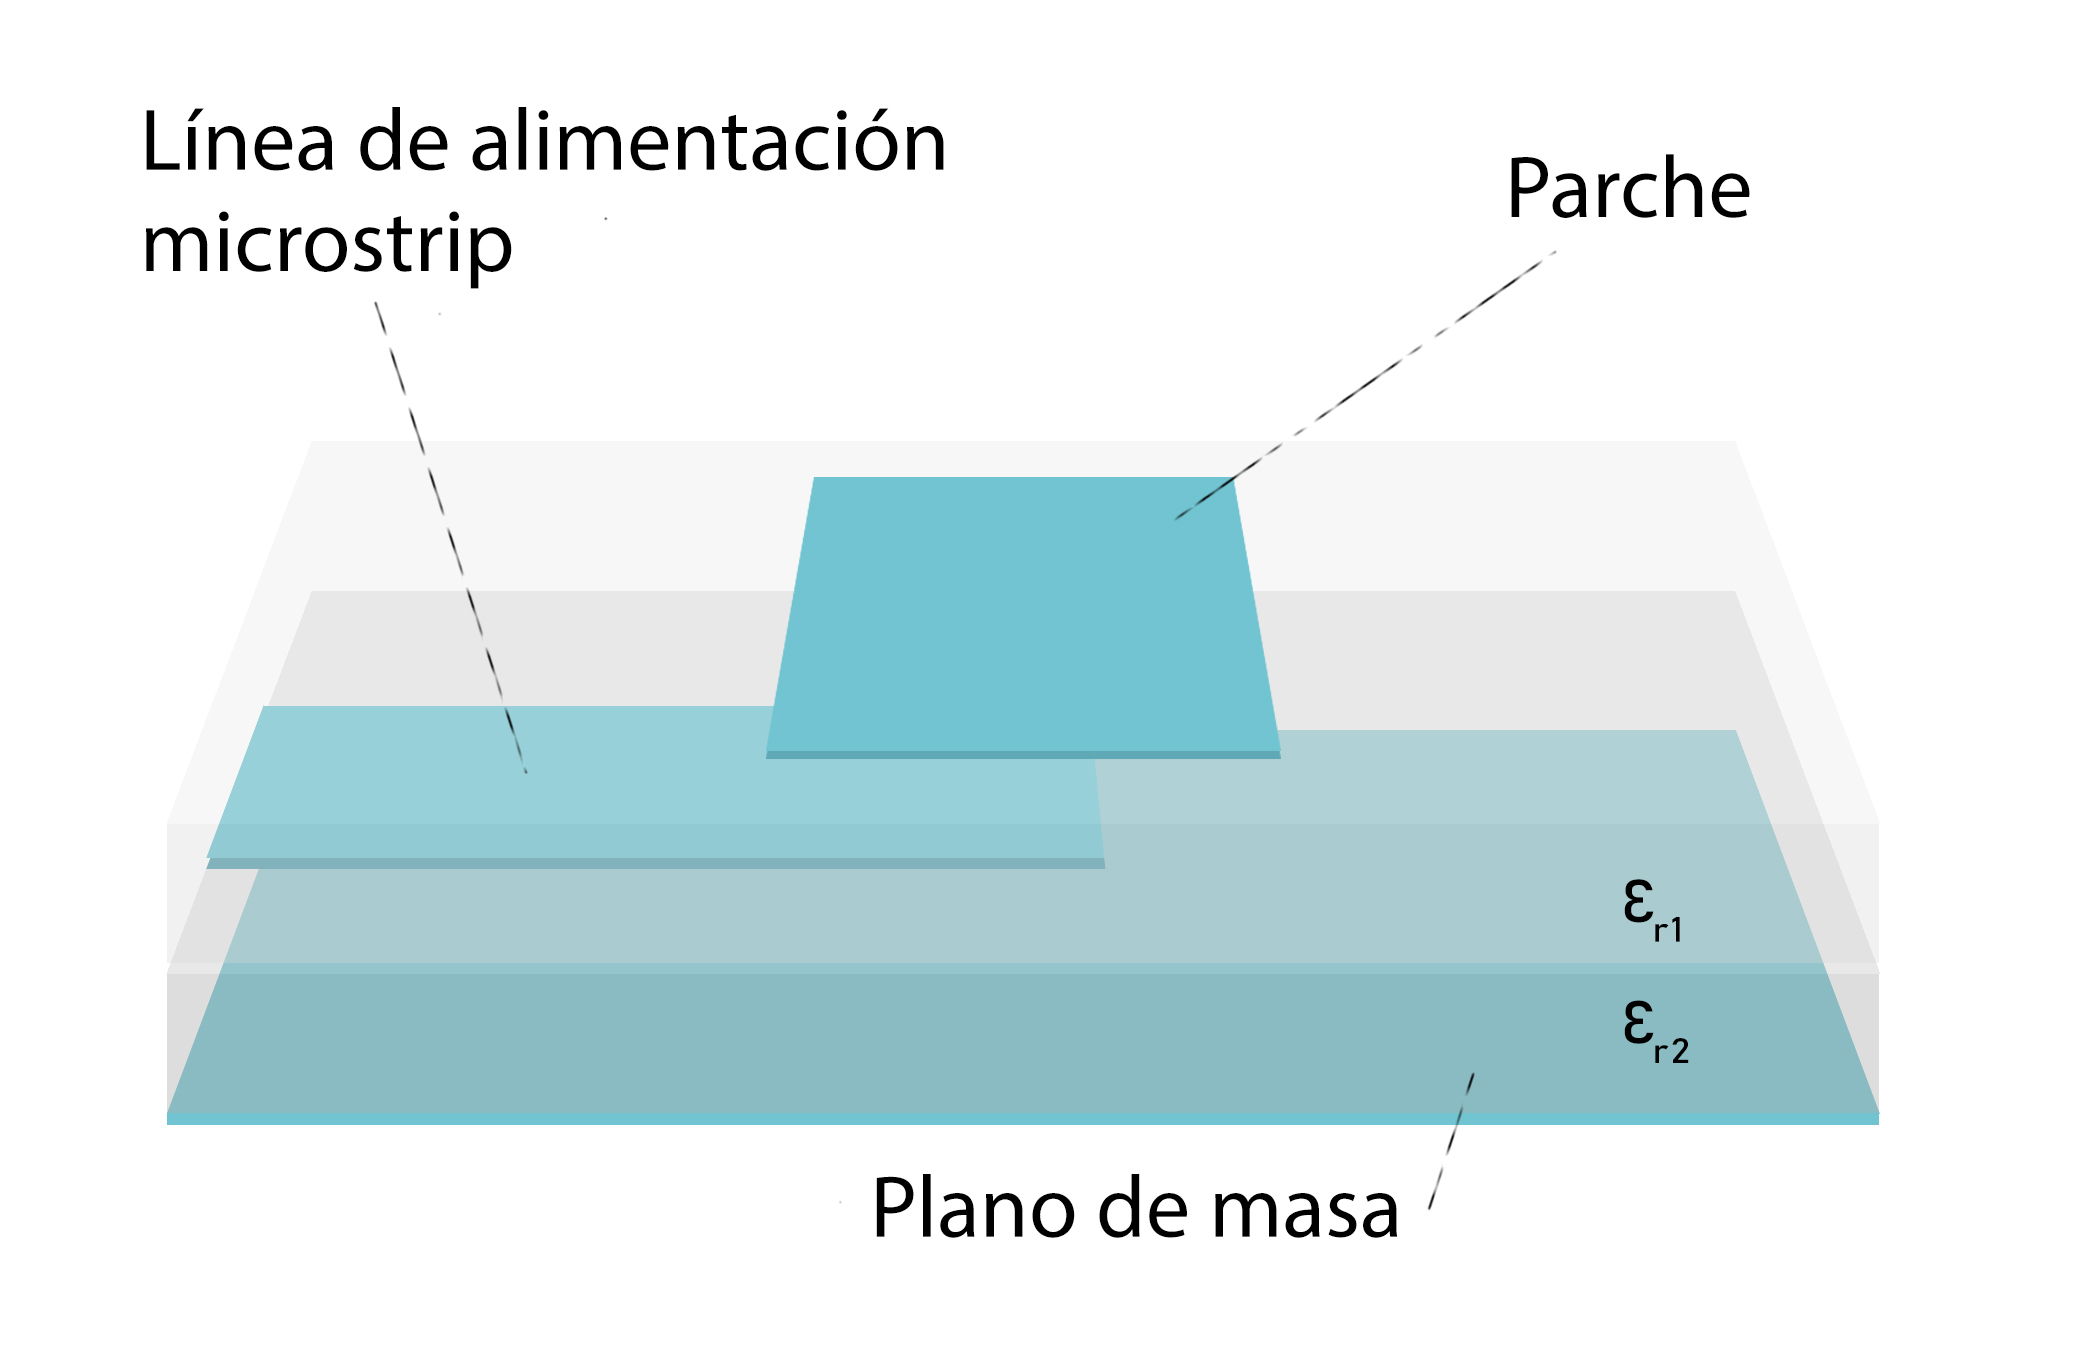
\includegraphics[width=\textwidth]{archivos/parche/proximidad}
         \caption{Alimentación por proximidad}
         \label{fig:proximidad}
     \end{subfigure}
     \hfill
     \begin{subfigure}[b]{0.45\textwidth}
         \centering
         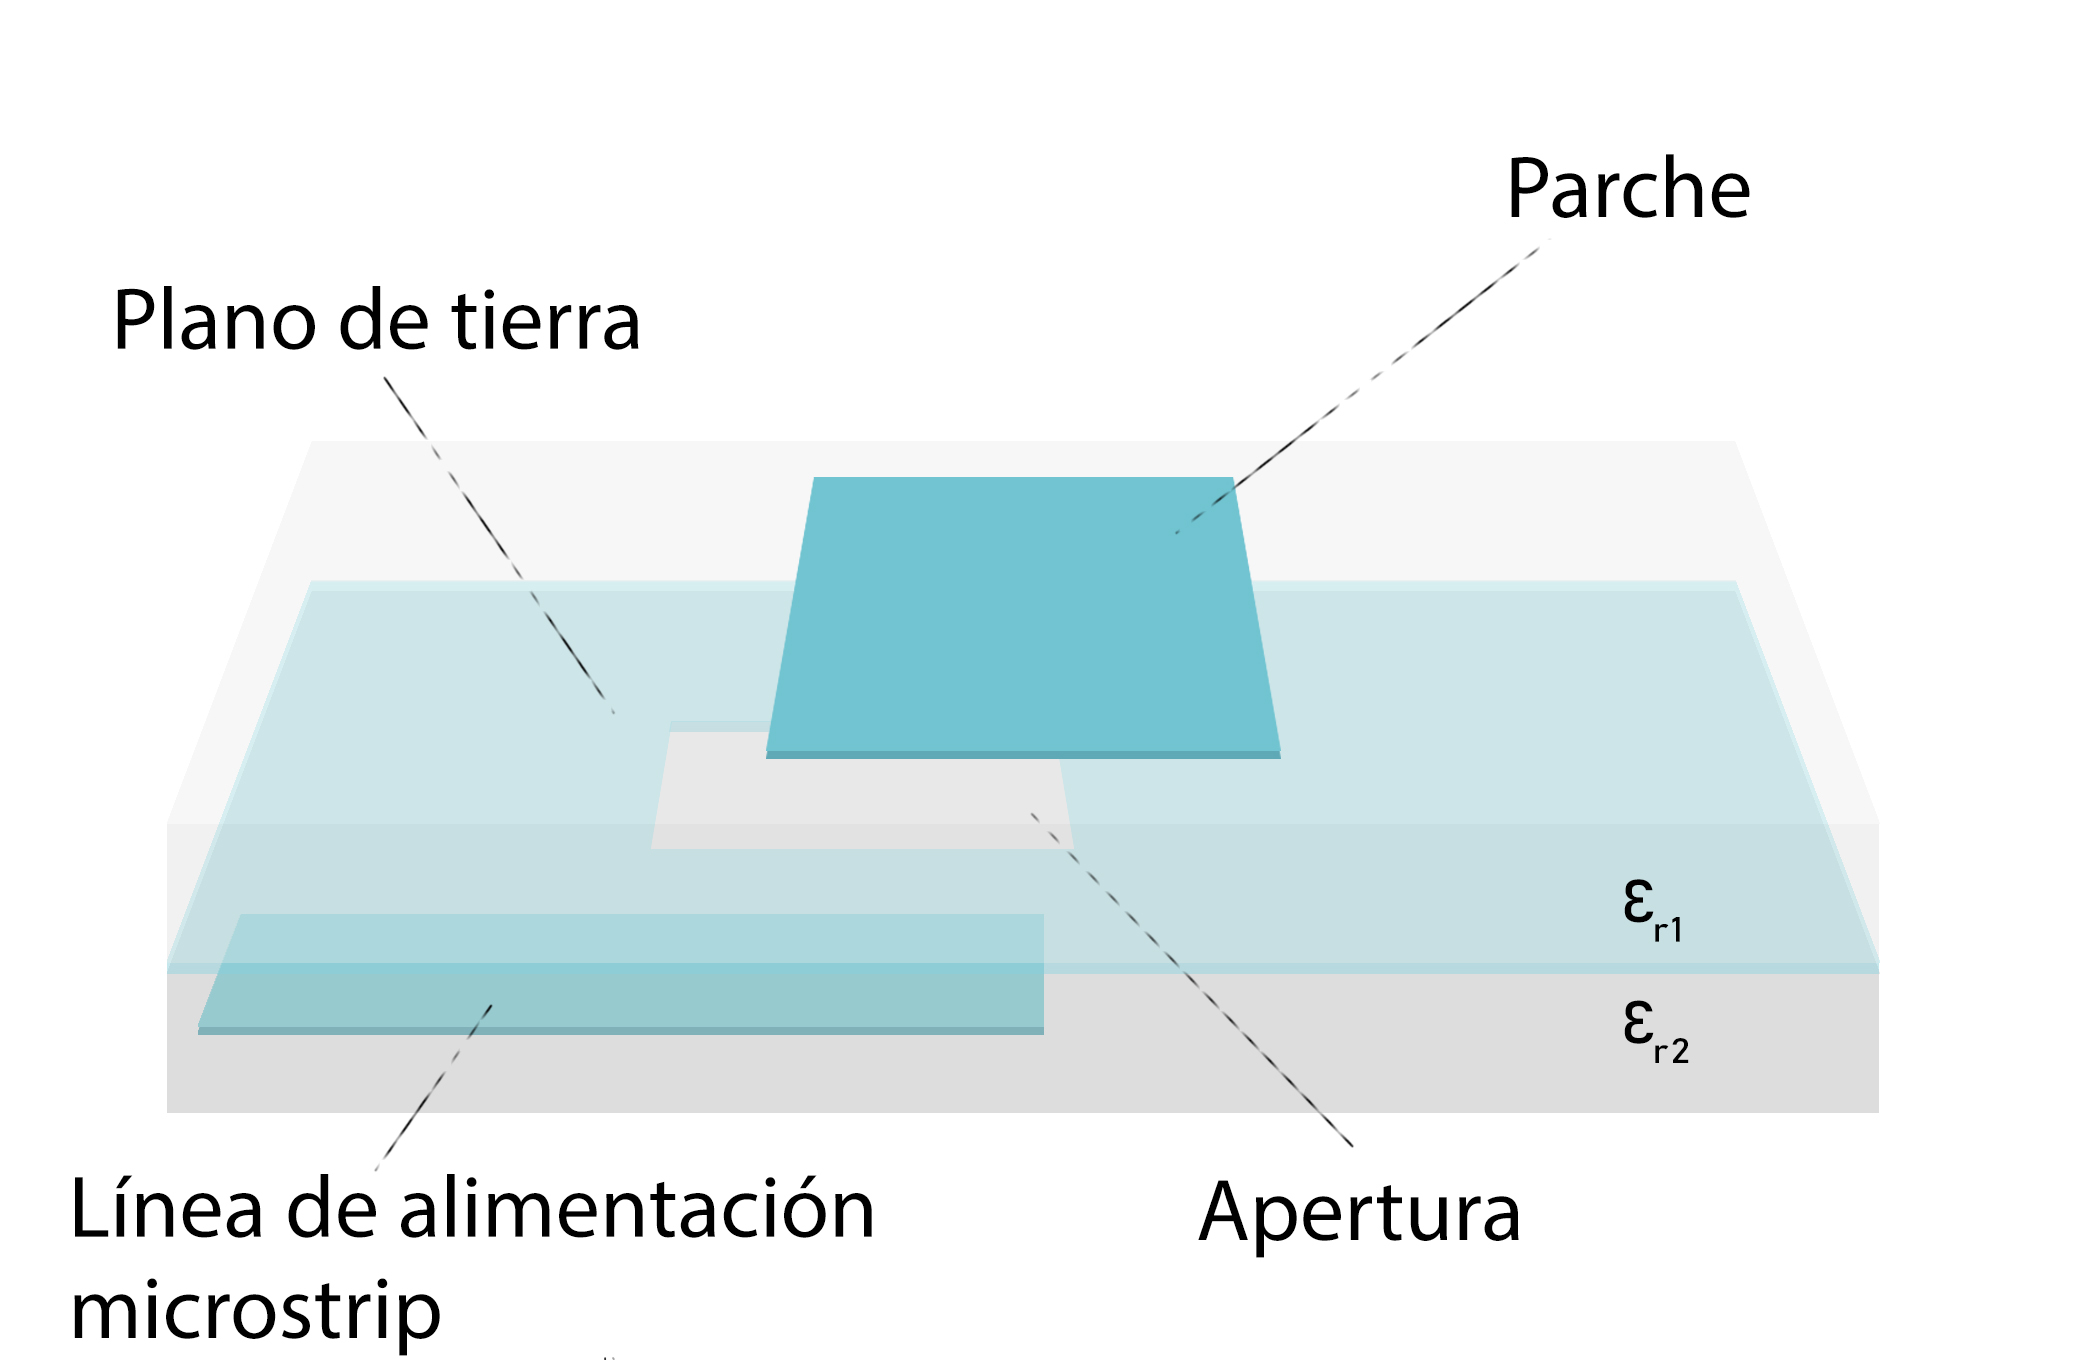
\includegraphics[width=\textwidth]{archivos/parche/apertura}
         \caption{Alimentación por ranura}
         \label{fig:ranura}
     \end{subfigure}
        \caption{Tipos de alimentación de antenas microstrip.}
        \label{fig:sistemas}
\end{figure}

\begin{table}[H]
   

   \small % text size of table content
   \centering % center the table
   \begin{tabular}{m{0.2\linewidth}m{0.15\linewidth}m{0.15\linewidth}m{0.15\linewidth}m{0.15\linewidth}} % alignment of each column data
   \toprule[\heavyrulewidth]\toprule[\heavyrulewidth]
   \textbf{Característica} & \textbf{Linea Microstrip} & \textbf{Sonda Coaxial} & \textbf{Proximidad} & \textbf{Ranura} \\ 
   \midrule
   \textbf{Radiación del Feed} & Poca & Poca & Poca & Mínima \\
   \textbf{Fiabilidad} & Máxima & Alta & Alta & Alta \\
   \textbf{Fabricación} & Fácil & Requiere soldadura & Requiere alineación & Requiere alineación \\
   \textbf{Adaptación de impedancias} & Fácil & Fácil & Fácil & Fácil \\
   \textbf{Ancho de Banda} & 2-5\% & 2-5\% & 2-5\% & 13-15\% \\
   
   \bottomrule[\heavyrulewidth] 
   \end{tabular}
   \caption{Resumen de características de cada tipo de alimentación} 
      \label{tab:example}
\end{table}



\section{Métodos de análisis}
\label{analisis}
\par Existen diferentes métodos para analizar el comportamiento de una antena en tecnología microstrip. Cada uno ofrece una diferente relación entre complejidad y precisión entre los resultados empíricos y los que se obtienen en la realidad. Los métodos más comunes de análisis son el método  de línea de transmisión, el método de cavidad, y el método de onda completa. 
\\
\par El método de línea de transmisión es más sencillo pero con una menor exactitud a la hora de obtener los resultados así como una menor facilidad para modelar el acoplamiento. Este método además, solo es útil a la hora de diseñar y analizar parches rectangulares. Comparado con el, el método de cavidad ofrece una mayor precisión sacrificando la complejidad a la hora de realizar los cálculos. El método de onda completa es usado para obtener los resultados más exactos, versátiles, y con mayor facilidad para tratar elementos finitos, así como arrays infinitos, pilas, y antenas microstrip con formas completamente aleatorias, pero sacrificando la facilidad en el análisis ya que se trata de un método muy complejo y no ofrece una buena visión física para entender los fenómenos físicos que ocurren en la antena. 
\\
\par En este proyecto se ha usado principalmente el método de línea de transmisión para el diseño de las antenas microstrip, con lo que se procederá a profundizar en la explicación de este método obviando los métodos de cavidades y onda completa dada su complejidad. \cite{Balanis2015}

\subsection{Método de análisis y diseño por línea de transmisión}
\label{351}
\par El método de línea de transmisión, es un método de análisis del comportamiento físico de una antena microstrip que ofrece una manera sencilla de modelar la antena, con unos cálculos más rápidos y una visión más sencilla de lo que ocurre físicamente en la antena, a costa de unos resultados menos precisos que los que encontraríamos en otros métodos de análisis. Este método de análisis modela la antena microstrip como dos ranuras, separadas por una línea de transmisión de baja impedancia $Z_{c}$ y de longitud \textit{L} (fig. \ref{fig:modelo}). 
\\

\begin{figure}[h]
    \centering
        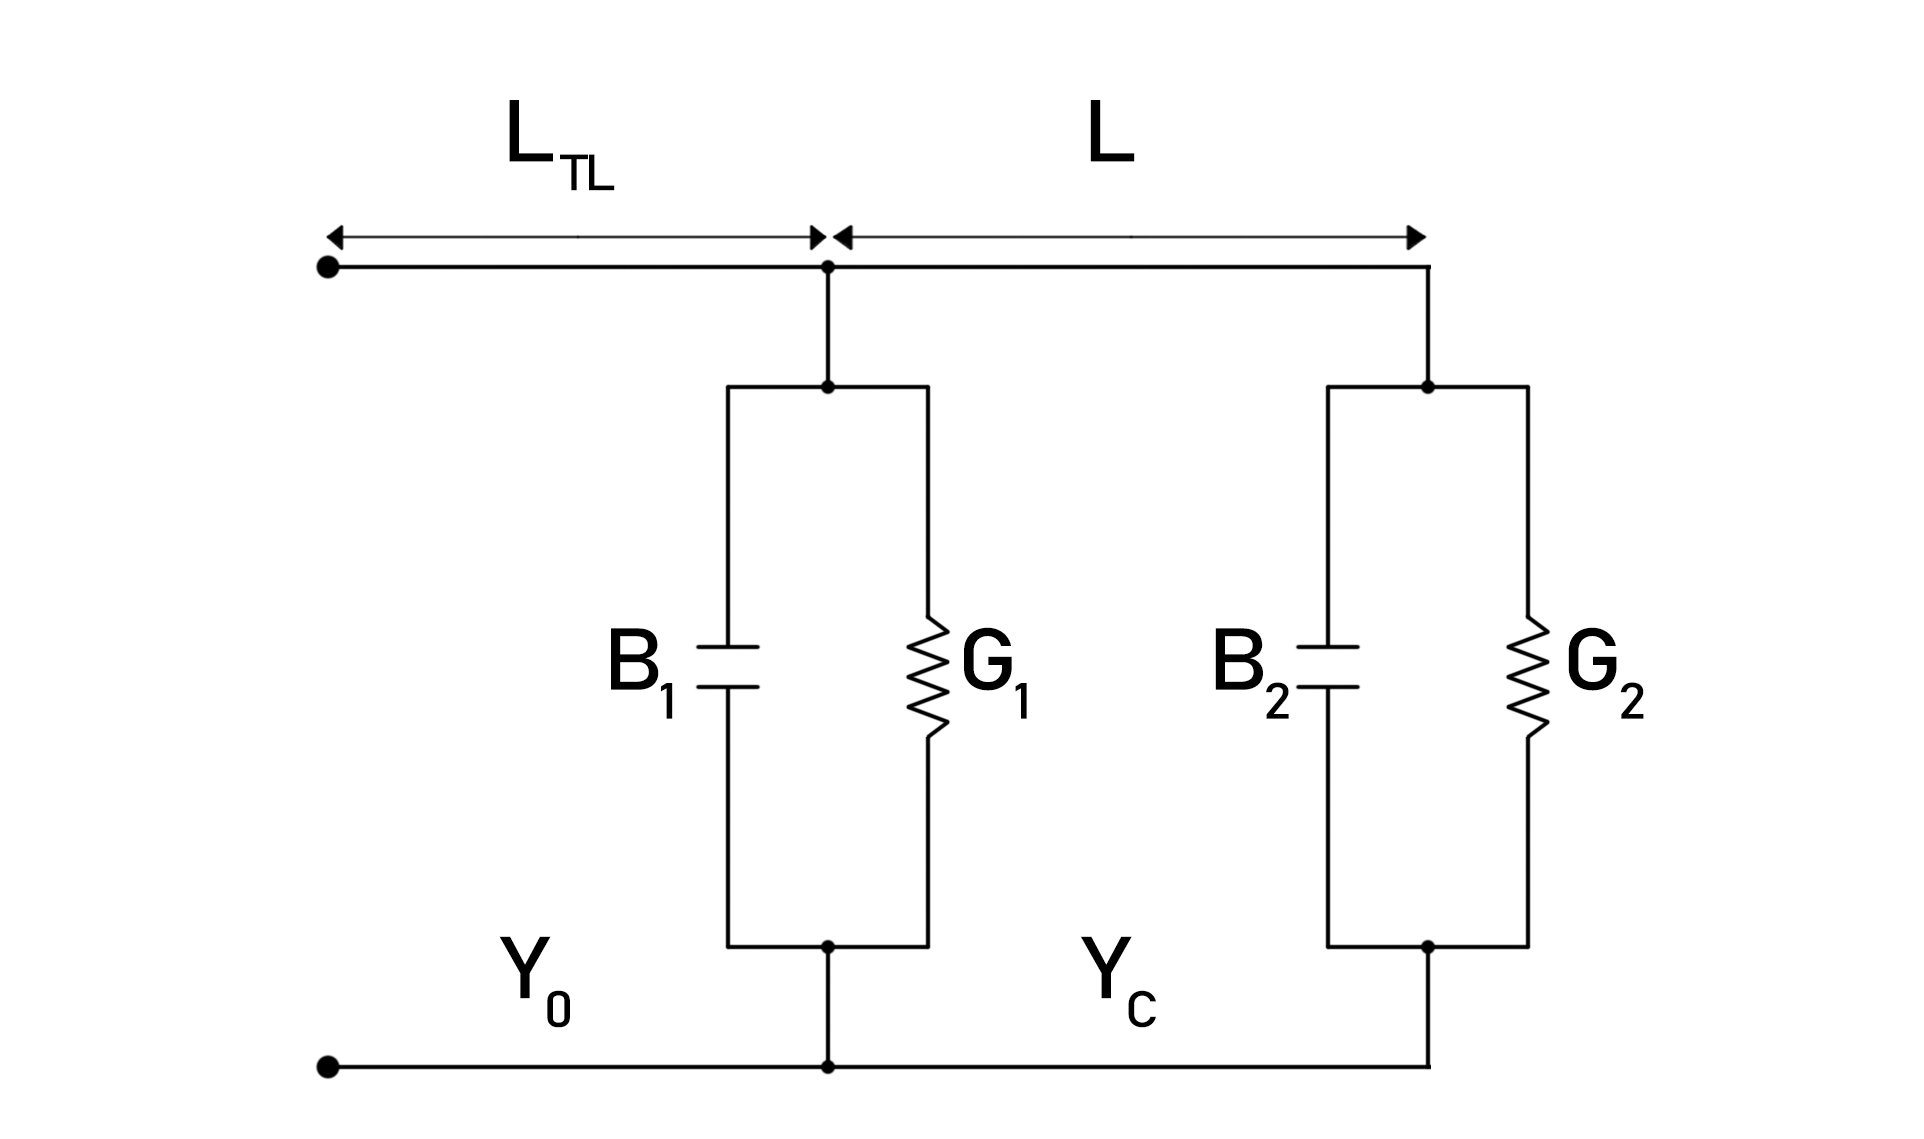
\includegraphics[width=12cm]{archivos/parche/circuito}
        \caption{Modelo equivalente del circuito de la antena microstrip.}
        \label{fig:modelo}
\end{figure}

\par Para explicar el modelo de línea de transmisión tomaremos como ejemplo el análisis de un parche rectangular. Debido a que las longitudes de ancho \textit{W} y alto \textit{L} del parche son limitadas, los campos eléctricos en los ejes producen el efecto \textit{fringing} en el parche. Este efecto es de vital importancia a la hora del diseño de las dimensiones de los ejes ya que influye en la frecuencia de resonancia de la antena. Para el plano E, el efecto \textit{fringing} se comporta en función de la relación entre la longitud del parche \textit{L} y la altura del substrato \textit{h} y su constante dieléctrica \textit{$\varepsilon_{r}$}. 
\\
\par  Para el caso en el que la antena original se sustenta sobre el plano superior de un substrato con dieléctrico \textit{$\varepsilon_{r}$} y y por encima del parche solo se encuentra el aire, se puede observar cómo el flujo de las líneas de campo eléctrico viajan en primer lugar por el aire, para luego concentrar su flujo en el substrato (fig. \ref{fig:fringing}). Esto hace que la antena se pueda modelar como una línea microstrip sumergida en un substrato cuya constante dieléctrica es $\varepsilon_{reff}$, también denominada \textit{constante dieléctrica efectiva} (fig. \ref{fig:ereff}). Se puede obtener la constante dieléctrica efectiva mediante la ecuación \ref{eq:ereff}.

\begin{figure}[h]
     \centering
     \begin{subfigure}[b]{0.7\textwidth}
         \centering
         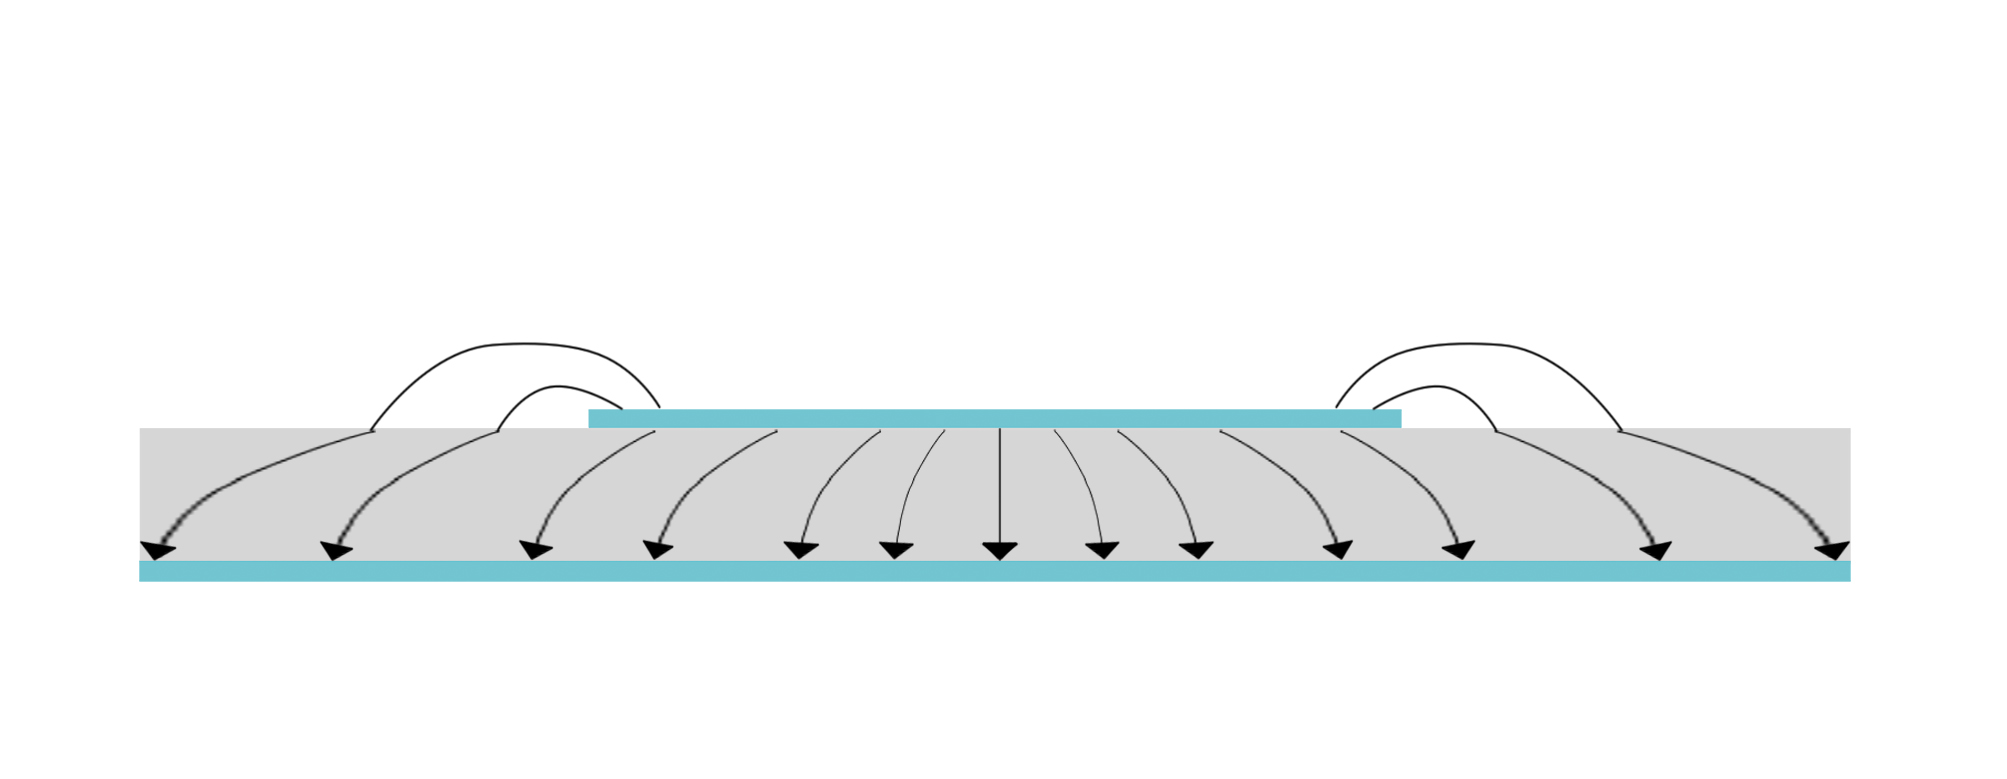
\includegraphics[width=\textwidth]{archivos/parche/Fringing}
         \caption{Distribución de las líneas de campo eléctrico}
         \label{fig:fringing}
     \end{subfigure}
     \hfill
     \begin{subfigure}[b]{0.7\textwidth}
         \centering
         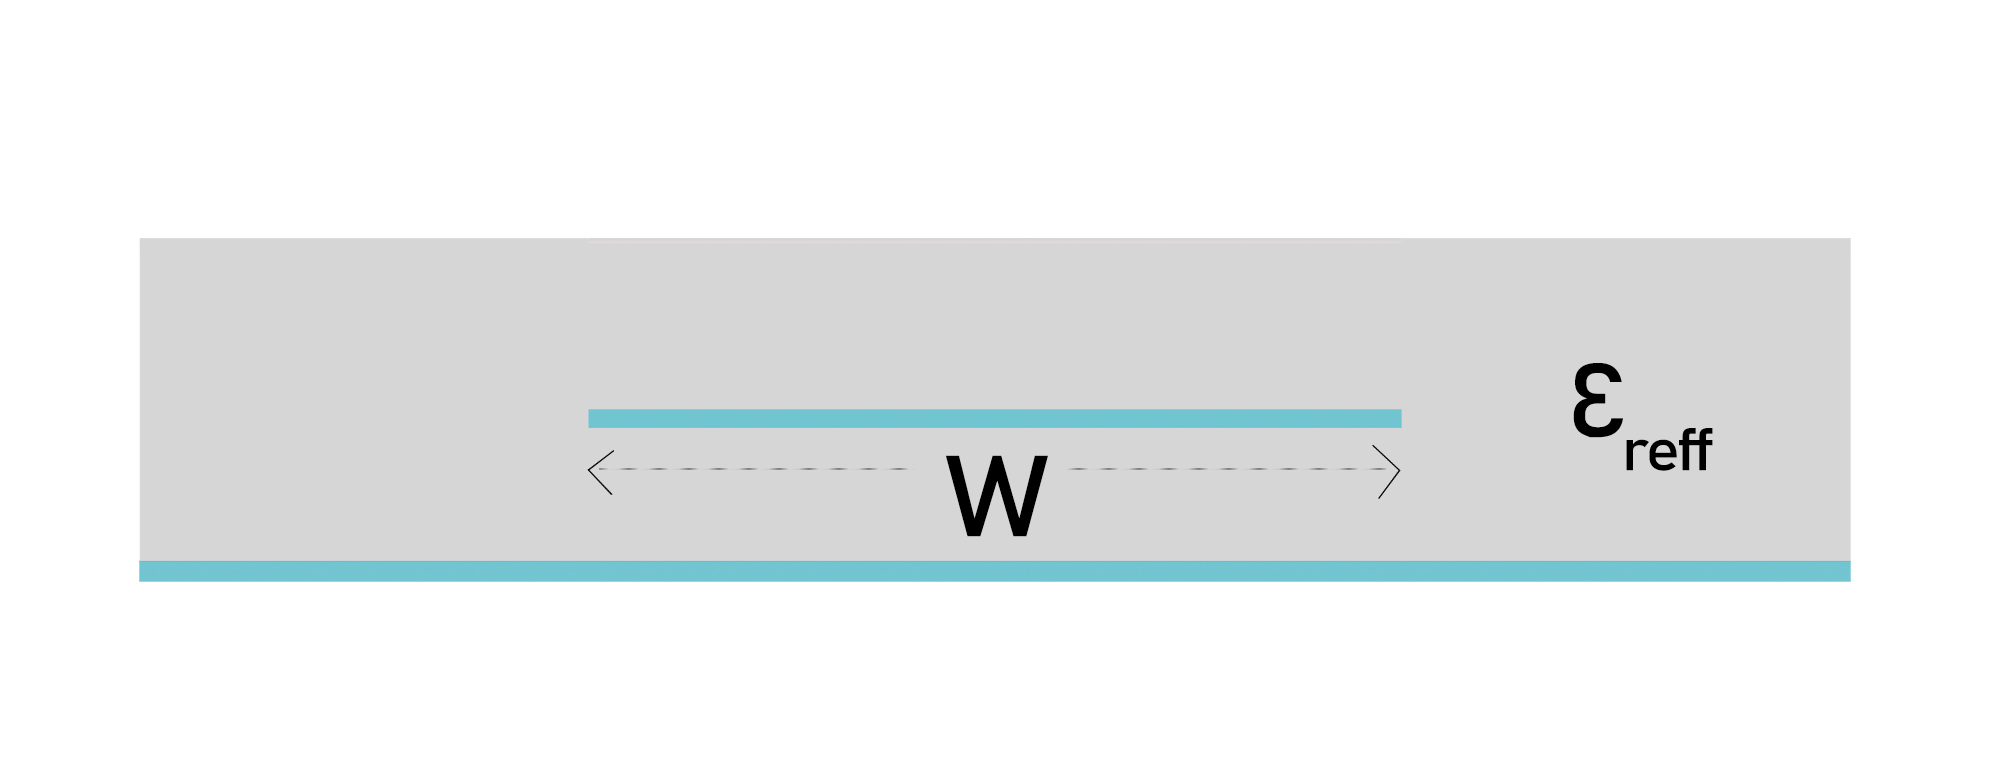
\includegraphics[width=\textwidth]{archivos/parche/ereff}
         \caption{Modelado de la constante dieléctrica efectiva}
         \label{fig:ereff}
     \end{subfigure}
     \hfill
        \caption{Antena microstrip según el modelo de línea de transmisión.}
        \label{fig:modelado}
\end{figure}

\begin{equation}
	\varepsilon _{reff}=\frac{\varepsilon _{r}+1}{2}+\frac{\varepsilon _{r}-1}{2}\left ( 1+\frac{12h}{W} \right )^{-\frac{1}{2}}
	\label{eq:ereff}
\end{equation}

\par En efectos prácticos, el efecto \textit{fringing} produce que las dimensiones eléctricas vistas por la antena sean mayores a las dimensiones físicas reales. Este incremento de distancia \textit{$\Delta$L} (fig. \ref{fig:modelado2}), queda en función de la constante dieléctrica efectiva $\varepsilon_{reff}$, y la relación entre la anchura y la altura de la antena (eq. \ref{eq:deltal}). El hecho de añadir este incremento de longitud hará que los cálculos respecto al diseño de la antena tengan que estar en función de esta nueva longitud (eq. \ref{eq:leff}).

\begin{figure}[h]
     \centering
     \begin{subfigure}[b]{0.7\textwidth}
         \centering
         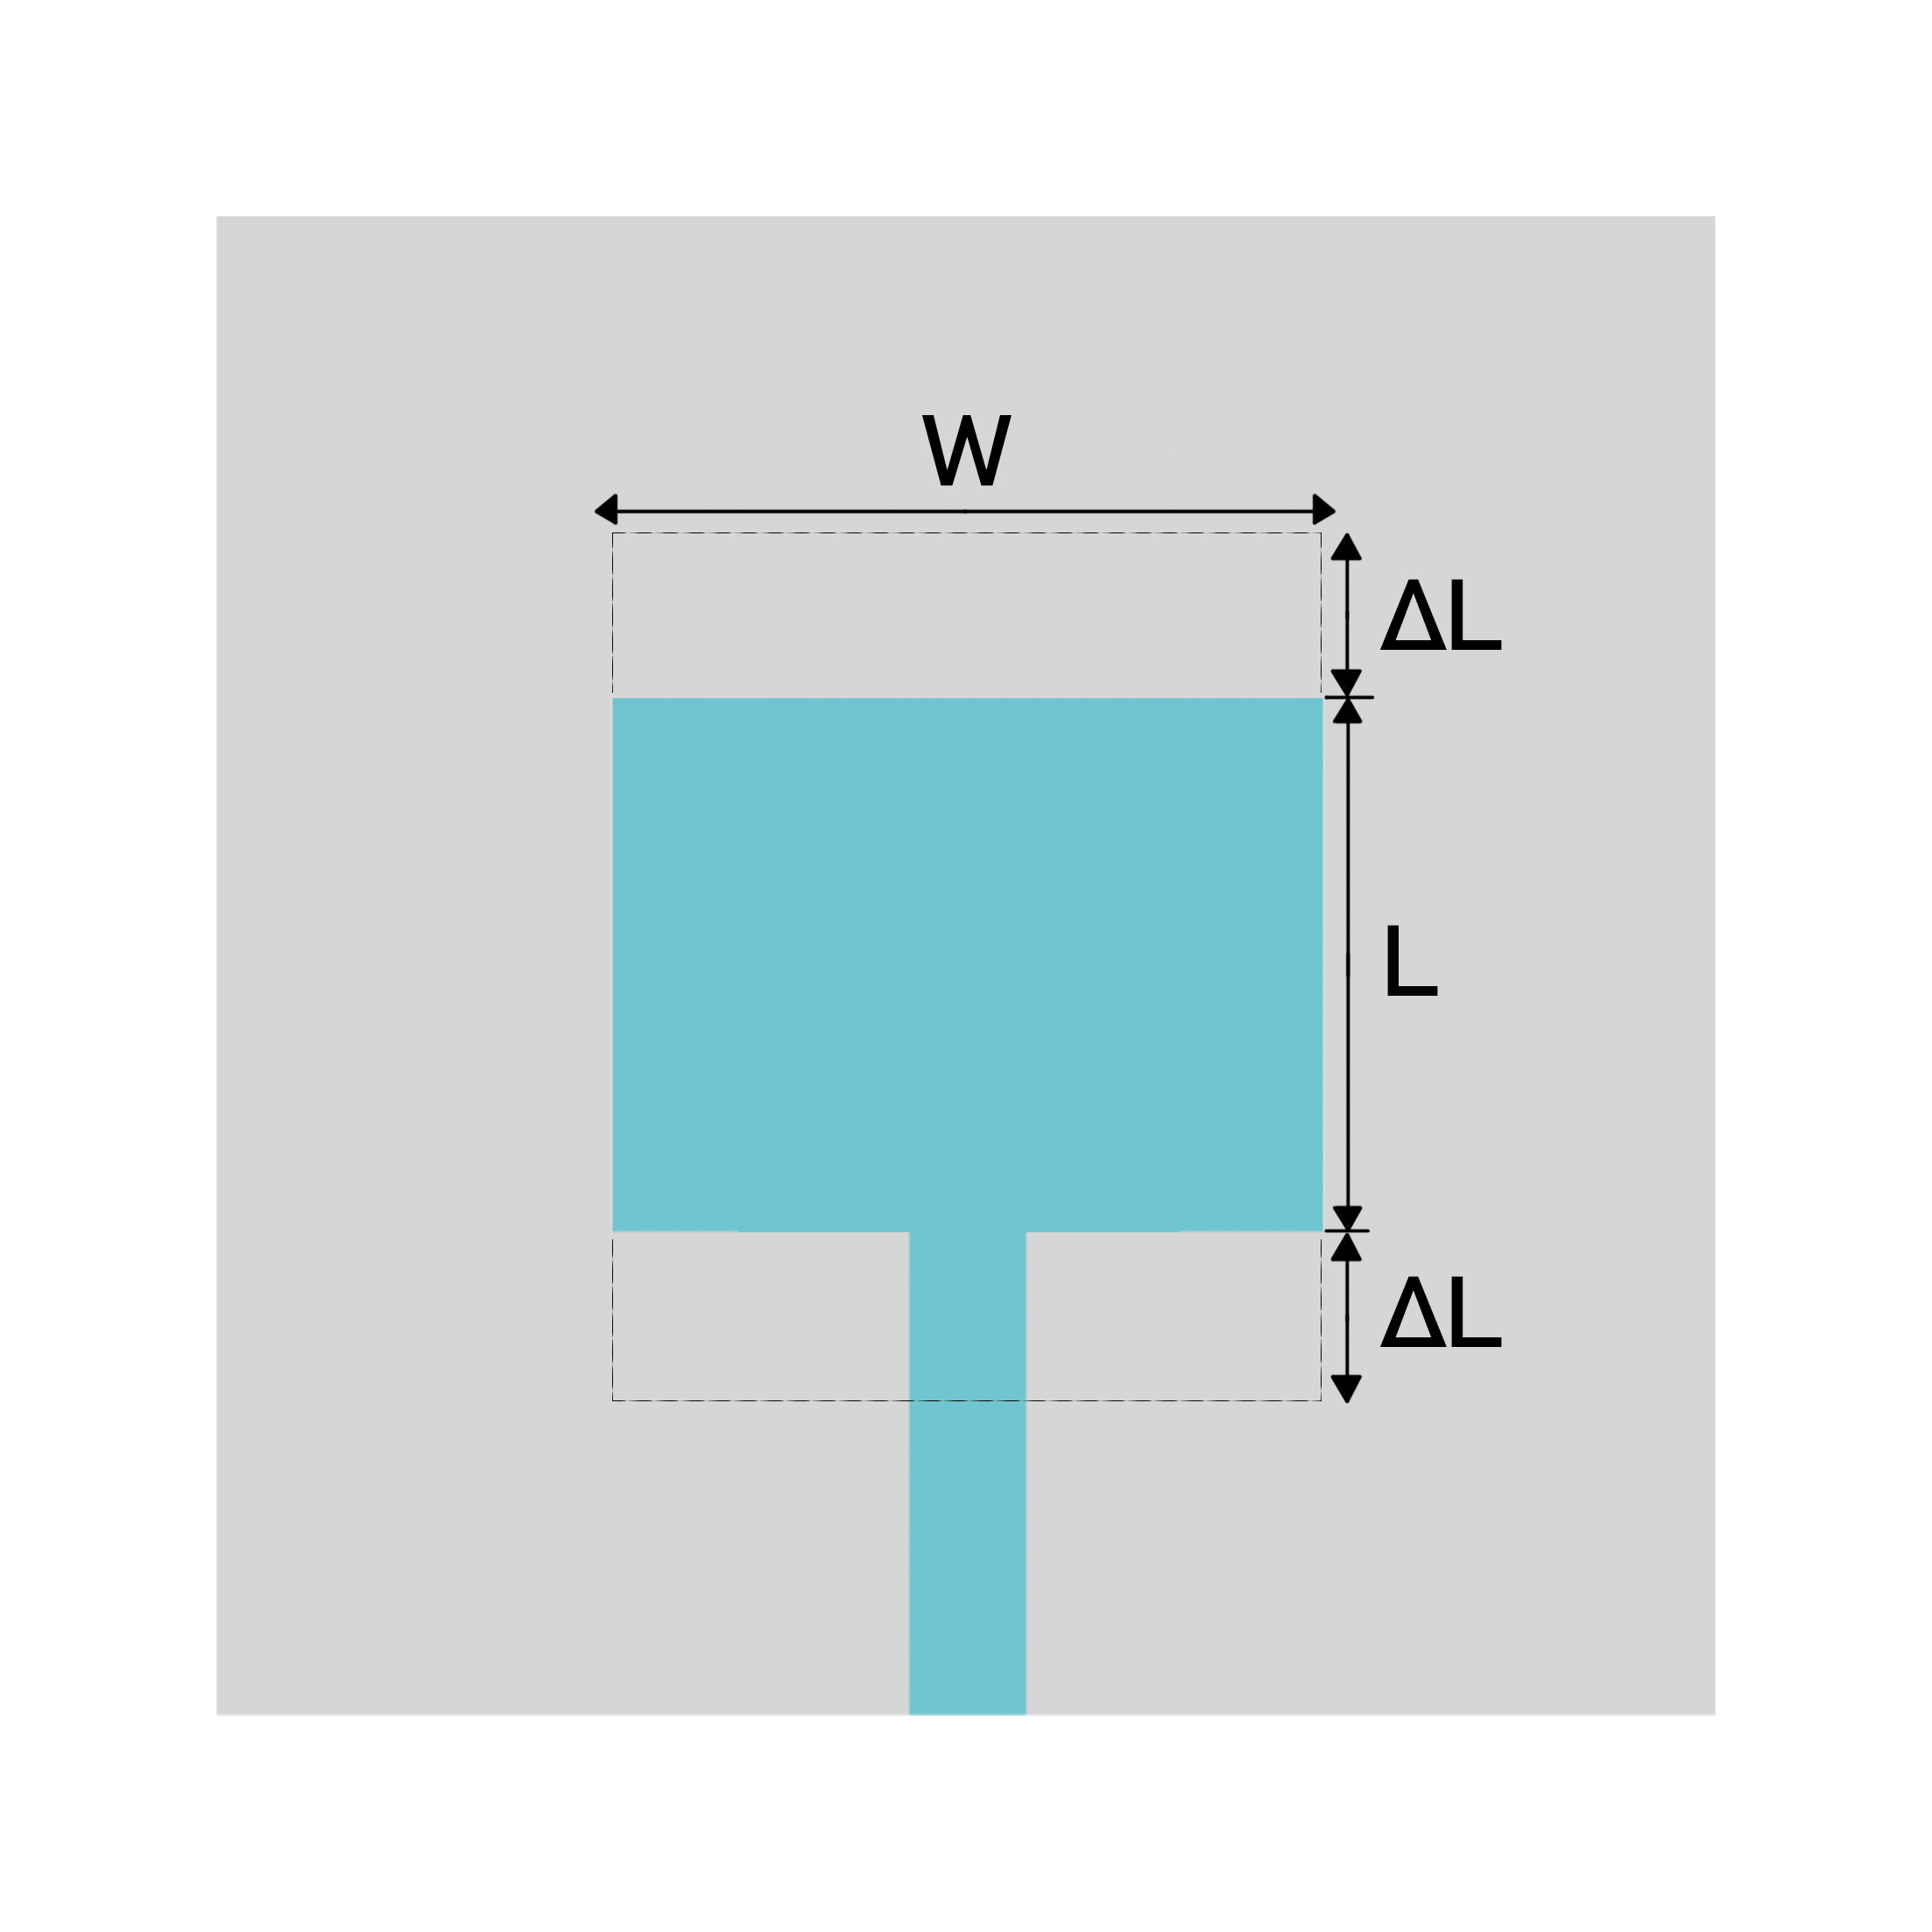
\includegraphics[width=\textwidth]{archivos/parche/efectivelength2}
         \caption{Vista de alzado}
         \label{fig:planta}
     \end{subfigure}
     \hfill
     \begin{subfigure}[b]{0.7\textwidth}
         \centering
         
\includegraphics[width=\textwidth]{archivos/parche/efectivelength}
         \caption{Vista de perfil}
         \label{fig:perfil}
     \end{subfigure}
     \hfill
        \caption{Modelado del incremento de longitud debido al efecto \textit{fringing}.}
        \label{fig:modelado2}
\end{figure}

\begin{equation}
	\frac{\Delta L}{h}=0.412\frac{(\varepsilon _{reff}+0.3)(\frac{W}{h}+0.264)}{(\varepsilon _{reff}-0.258)(\frac{W}{h}+0.8)}
	\label{eq:deltal}
\end{equation}

\begin{equation}
	L_{eff}=L+2\Delta L
	\label{eq:leff}
\end{equation}

\par Otra variable que será importantes a la hora de diseñar la antena o el array de antenas será la longitud de onda en el medio guiado $\lambda_{g}$:

\begin{equation}
	\lambda_{g}=\frac{\lambda_{0}}{\sqrt{\varepsilon _{reff}}}
	\label{eq:lambdaguided}
\end{equation}


\par Una vez que se ha tenido en cuenta los conceptos de longitud efectiva y \textit{fringing} se puede proceder al diseño del parche microstrip. Se trata de un proceso de diseño sencillo según el método de línea microstrip, en el cual solo necesitaremos especificar de antemano los valores de constante dieléctrica del substrato elegido $\varepsilon_{r}$, la altura de este \textit{h} y la frecuencia a la que se pretende que trabaje la antena \textit{$f_{r}$}. Con estos parámetros se calcularan las dimensiones del parche \textit{W} y \textit{L}. Para ello es común seguir el siguiente flujo de trabajo:

\begin{enumerate}
  \item Calcular la anchura del parche \textit{W}:
  \begin{equation}
	W=\frac{1}{2f_{r}\sqrt{\mu _{0}\varepsilon _{}0}}\sqrt{\frac{2}{\varepsilon _{r}+1}}=\frac{v_{0}}{2f_{r}}\sqrt{\frac{2}{\varepsilon _{r}+1}}
	\label{eq:W}
\end{equation}

Donde $v_{0}$ es la velocidad de la luz en el vacío.

  \item Calcular la constante dieléctrica efectiva $\varepsilon_{reff}$ mediante la eq. \ref{eq:ereff}.
  
  \item Calcular el incremento de longitud debido al efecto \textit{fringing} mediante la ecuación \ref{eq:deltal}.
  
  \item Finalmente obtener la longitud del parche \textit{L}:
  
   \begin{equation}
	L=\frac{1}{2f_{r}\sqrt{\varepsilon _{reff}}\sqrt{\mu _{0}\varepsilon _{}0}}-2\Delta L
	\label{eq:L}
\end{equation}
\end{enumerate}

\par Una vez que se han calculado las dimensiones del parche, vamos a proceder a su adaptación. Para ello, es muy común el uso de pequeñas inserciones de la línea de alimentación microstrip o \textit{inset}  dentro del parche, abriendo dos ranuras alrededor de esta. Con esto se consigue que la línea de alimentación con una impedancia característica $Z_{c}$ este completamente adaptada en impedancias con el parche. Estas pequeñas ranuras tendrán una longitud específica en la que se sabe que la posición en la que se encuentra el final de la línea concuerda con la misma impedancia dentro del parche.
\\
\par Para hallar la longitud del \textit{inset} se necesita tener en cuenta las admitancias \textit{Y}, conductancias \textit{G} y susceptancias \textit{B} de las ranuras y así poder calcular cuál es la resistencia de entrada resonante donde buscar la adaptación entre \textit{feed} y parche. Para ello primero se calcula la conductancia \textit{$G_{1}$}:
\\
\begin{equation}
	G_{1}=\frac{I_{1}}{120\pi^{2}}
	\label{eq:g1}
\end{equation}

\par Donde \textit{$I_{1}$} se calcula mediante:

\begin{equation}
	I_{1}=\int_{0}^{\pi}\left [ \frac{\sin(\frac{k_{0}W}{2})\cos\theta } {\cos\theta} \right ]^{2}\sin^{3}\theta d\theta
	\label{eq:I1}
\end{equation}

\par Las dos ranuras  producirán una conductancia mutua \textit{$G_{12}$} cuyos efectos han de ser tenidos en cuenta para calcular la resistencia de entrada.

\begin{equation}
	G_{12}=\frac{I_{12}}{120\pi^{2}}
	\label{eq:g12}
\end{equation}

\par Donde \textit{$I_{12}$} se calcula mediante:

\begin{equation}
	I_{12}=\int_{0}^{\pi}\left [ \frac{\sin(\frac{k_{0}W}{2})\cos\theta } {\cos\theta} \right ]^{2} J_{0}(k_{0}L\sin(\theta)) 
 \sin^{3}\theta d\theta
	\label{eq:I12}
\end{equation}

Donde se entiende como \textit{$J_{0}$} la función de Bessel de orden cero.
\\
\par A continuación, se obtendrá la resistencia de entrada resonante \textit{$R_{in}$} mediante:

\begin{equation}
	R_{in}=\frac{1}{2(G_{1}\pm G_{12})}
	\label{eq:rin}
\end{equation}

\par Finalmente, hallaremos la distancia con la que se ha de diseñar el  \textit{inset} \textit{$y_{0}$} (fig. \ref{fig:inset}),  para conseguir la adaptación de impedancias entre la alimentación directa por línea microstrip y el parche.

\begin{equation}
	y_{0}=\left ( \frac{L}{\pi} \right )\arccos\left ( \sqrt{\frac{R_{in}(y=y_{0})}{R_{in}}} \right )
	\label{eq:yo}
\end{equation}

Donde \textit{$R_{in}(y=y_{0})$} es la impedancia característica de la línea de alimentación microstrip.

\begin{figure}[h]
    \centering
        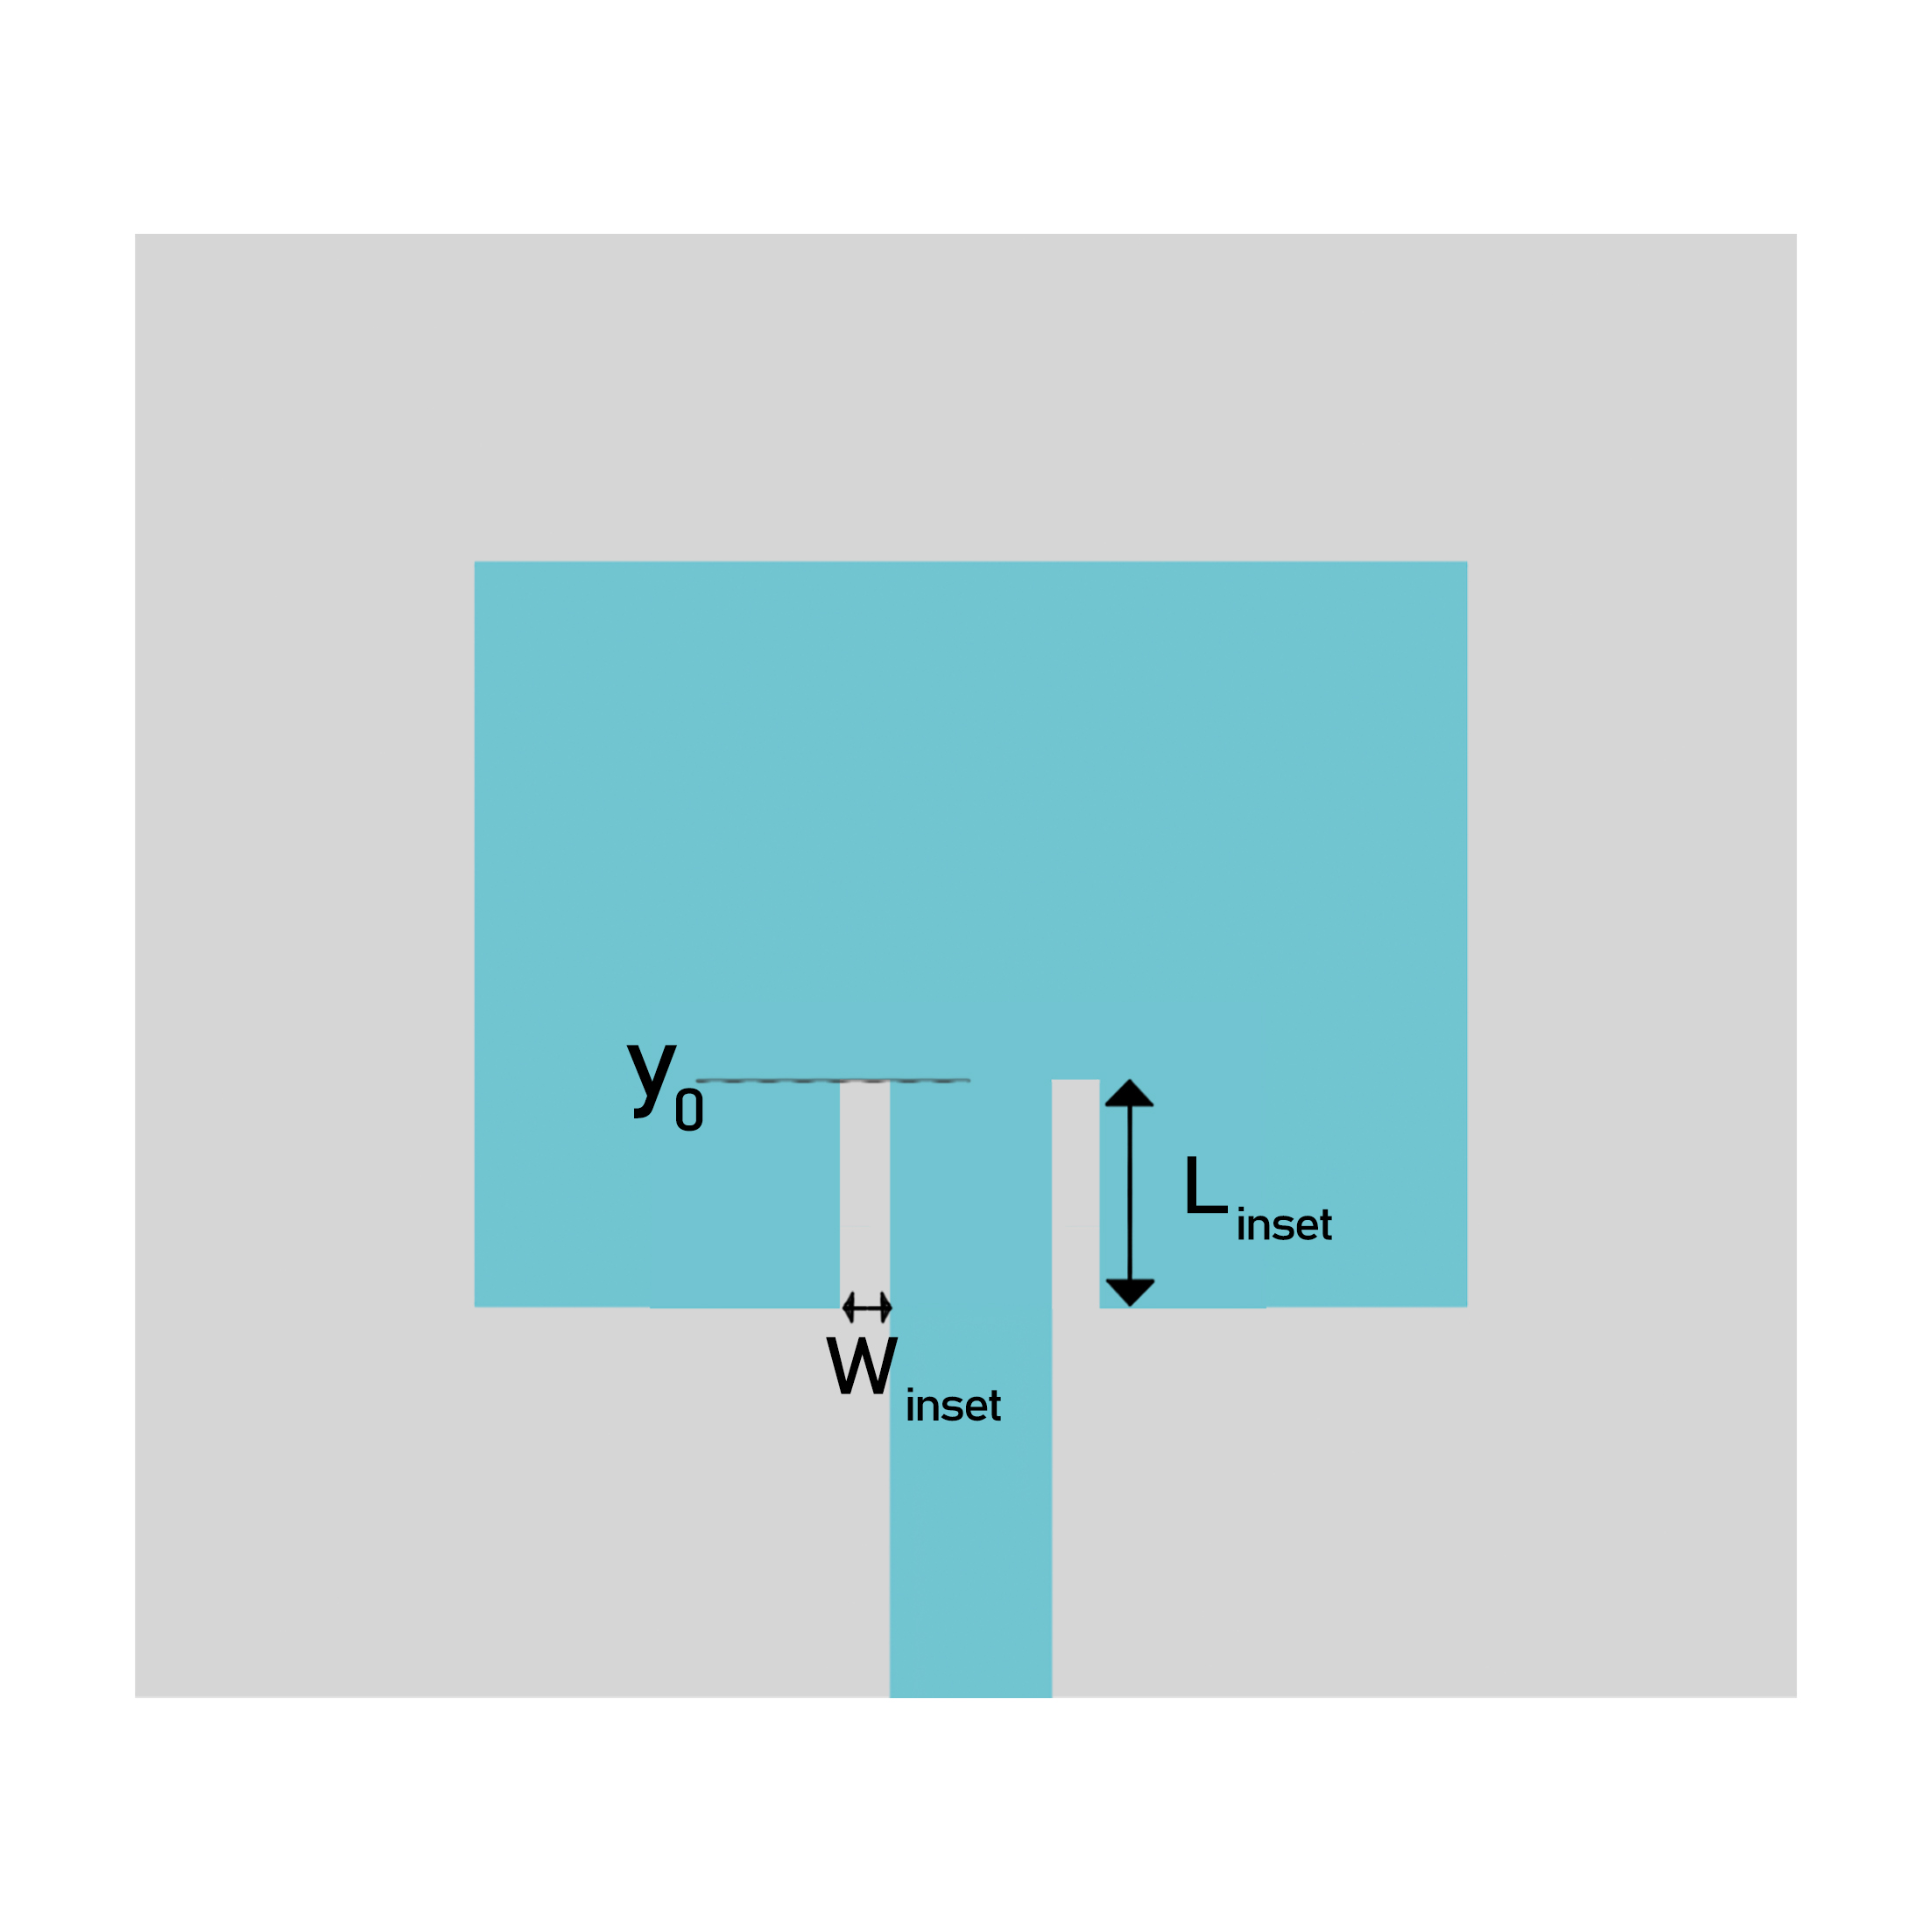
\includegraphics[width=0.7\textwidth]{archivos/parche/inset}
        \caption{Altura del \textit{inset} para adaptar las impedancias.}
        \label{fig:inset}
\end{figure}

\par Tras realizar el análisis se obtendrán unos parámetros de pérdidas de retorno de la antena con leves margenes de error sobre los inicialmente buscados en el diseño. Esto se debe a la simpleza de análisis del modelo de línea de transmisión, pero estos parámetros ya estarán dentro de los órdenes de magnitud buscados y se hará muy sencilla la corrección de ciertas dimensiones para conseguir adaptar el diseño del todo a nuestras especificaciones.

\section{Otros parámetros de análisis}
\par Además de los parámetros que se han calculado anteriormente para diseñar la antena microstrip, la construcción del sistema completo necesitará de otras características para su correcto funcionamiento. Estos nuevos parámetros están relacionados con las líneas de transmisión microstrip que alimentarán la antena y darán forma al array. Es importante que las líneas de transmisión tengas unas dimensiones específicas puesto que son estas las que definen sus características. Un buen diseño de las líneas de transmisión será de ayuda para una sencilla adaptación de impedancia entre la antena, la fuente y otras líneas de transmisión adyacentes. \cite{Balanis2015}

\subsection{Ancho de la línea de transmisión}
\par El ancho de la línea de transmisión $W_{feed}$ es clave para el diseño de esta puesto que es quien define su impedancia característica. En una configuración de línea de transmisión en tecnología microstrip, podemos sintetizar el ancho de la antena según la impedancia que se desea obtener para un diseño específico. Es necesario conocer de antemano cuál va a ser la altura del sustrato. A partir de ahí aplicaremos la siguiente ecuación:

\begin{equation}
	\frac{W_{feed}}{h}\approx \begin{cases}
\frac{8e^{A}}{e^{2A}-2}, & \frac{W_{feed}}{h}\leq 2
\\ \frac{2}{\pi}\left [ B-1-\ln(2B-1)+\frac{\varepsilon _{r}-1}{2\varepsilon _{r}}\left ( \ln(B-1)+0.39-\frac{0.61}{\varepsilon _{r}} \right ) \right ], & \frac{W_{feed}}{h}>  2
\end{cases}
	\label{eq:wh}
\end{equation}

\par Donde A y B pueden ser calculados mediante las ecuaciones:

\begin{equation}
	A=\frac{Z_{0}}{60}\sqrt\frac{\varepsilon_{r}+1}{2}+\frac{\varepsilon_{r}-1}{\varepsilon_{r}+1}\left ( 0.23+\frac{0.11}{\varepsilon_{r}} \right ) 
	\label{eq:A}
\end{equation}

\begin{equation}
	B=\frac{337\pi}{2Z_{0}\sqrt\varepsilon_{r}} 
	\label{eq:B}
\end{equation}

\par Donde $Z_{0}$ representa la impedancia que deseamos obtener en la línea de transmisión. Para que esta síntesis llegue a cumplirse, la altura o espesor de la línea de transmisión debe ser muy pequeña en comparación a las dimensiones de la anchura que se pretende obtener $W_{feed}$ y la altura del substrato donde se sostiene la tira microstrip \textit{h}.

\subsection{Altura de la línea de transmisión}
\par La altura o longitud $L_{feed}$ de la tira de alimentación microstrip puede, en principio, tener cualquier valor, y este queda reservado para nuestras necesidades de diseño. Pero existe un caso especial en el que es necesario especificar una altura de la línea concreta.

\subsubsection{Transformador $\lambda/4$}
\label{lambdacuartoscap}

\par Cuando, por razones de diseño de cualquier tipo de circuito electrónico, necesitamos realizar una adaptación de impedancias entre dos sistema cuyas impedancias son puramente reales u óhmicas y de distinto valor, existe un método de adaptación de estas, muy sencillo de implementar, denominado ``Transformador $\lambda/4$". 
\\
\par El transformador $\lambda/4$ se basa en la adición de una línea de transmisión cuya longitud sea igual a la cuarta parte de la longitud de onda en el medio guiado de la señal a la que se pretende transmitir. Esta línea de transmisión además deberá de tener una impedancia característica de:

\begin{equation}
	Z_{\lambda /4}=\sqrt{Z_{0}R_{L}}
	\label{eq:lambdacuartos}
\end{equation}

\par Donde $Z_{0}$ es la impedancia característica de la línea del circuito alimentador y $R_{L}$ es la carga del sistema que se desea adaptar al circuito anterior (fig. \ref{fig:lambdacuartos}).

\begin{figure}[h]
    \centering
        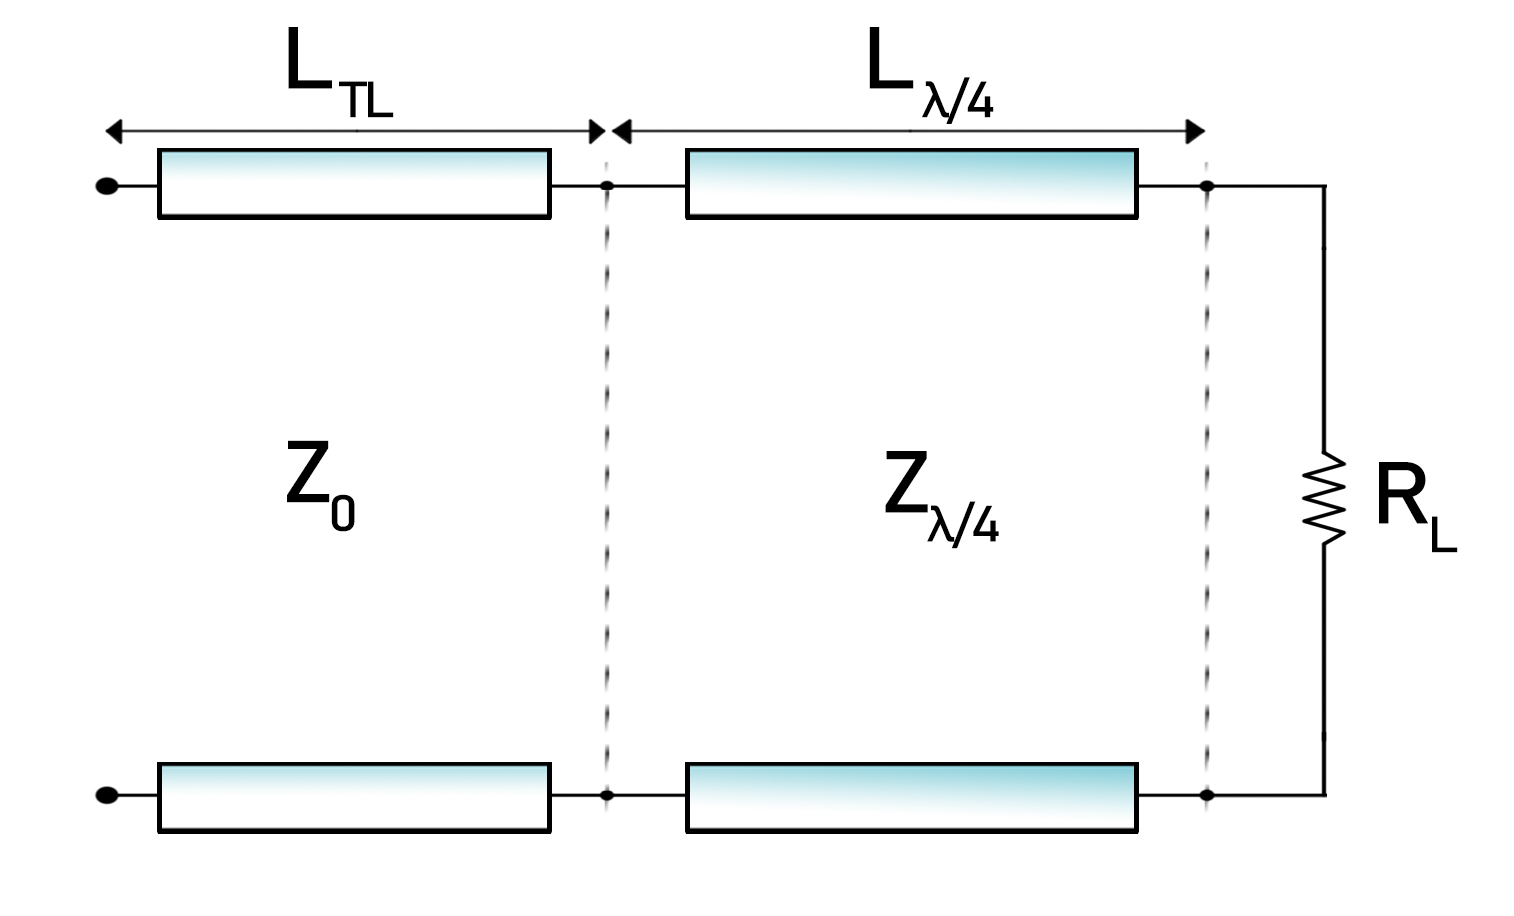
\includegraphics[width=\textwidth]{archivos/parche/lambda}
        \caption{Circuito con adaptador $\lambda/4$}
        \label{fig:lambdacuartos}
\end{figure}

\par En el caso de que cualquiera de las impedancias, ya sea de la parte del generador o de la carga, no sea puramente óhmica deberemos añadir otro tipo de adaptadores, como elementos pasivos en serie o paralelo, cuya función es anular la parte reactiva de las impedancias de estos circuitos. A lo largo del proceso de diseño y análisis de las antenas del proyecto, los transformadores $\lambda/4$ serán muy usados para la adaptación entre las líneas de 25, 50 y 100 $\Omega$ en las configuraciones de arrays donde la división de potencias en las bifurcaciones de caminos paralelos, impliquen el aumento de la impedancia de la línea, produciendo desadaptaciones finales con el parche que implicarían líneas de transmisión ínfimas para cumplir con los requerimientos de los divisores de potencia.


\begin{figure}[H]
    \centering
        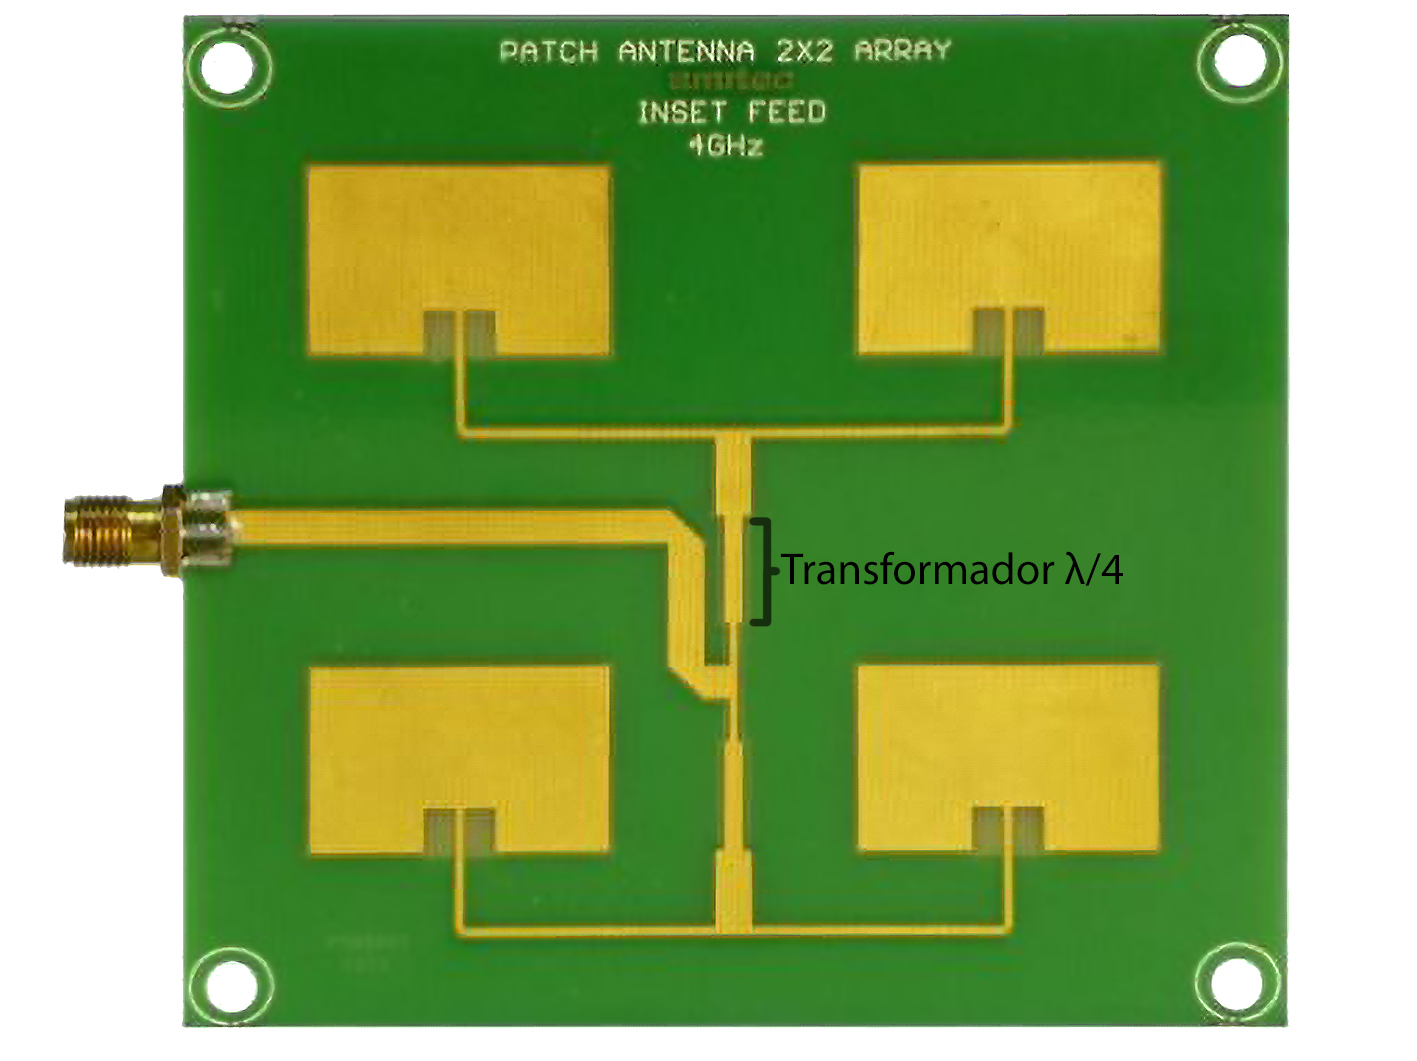
\includegraphics[width=\textwidth]{archivos/transformador}
        \caption{Ejemplo real de transformador $\lambda/4$ sobre un array microstrip 2x2 . \citep{Amitec2018}}
        \label{fig:transformador}
\end{figure}










